\documentclass[10pt,conference]{IEEEtran}
\usepackage[utf8]{inputenc}
\usepackage{booktabs,tabularx,graphicx,amsmath,amssymb,url,multirow}
\graphicspath{{figures/}}
\newcommand{\pfake}{P(\mathrm{FAKE})}
\title{LAVA: A Lightweight Benchmarking Framework for Robust and Real-Time Deepfake Voice Detection}
\author{Phan Khac Anh Tuan, Nguyen Phuong Chinh, Lai Thanh Dat, Nguyen Tan Khiem, and Truong Thanh Dat}
\begin{document}
\maketitle
\begin{abstract}
Deepfake-voice detectors are often compared under incompatible data, score, preprocessing, and runtime protocols. LAVA evaluates heterogeneous detectors through a common integrity, score, robustness, and timing contract while preserving native architectures. This interim study evaluates three locally trained Mel-sequence models and externally pretrained RawNet2 and AASIST checkpoints. SHA-256 grouping quarantined 30 byte-identical cross-label files. Clean evaluation used all 2,737 canonical test recordings. MobileNetV3Small-LSTM obtained F1 0.9724, AUC 0.9911, and EER 2.50\%; MnasNet-A1-LSTM obtained 0.9645, 0.9886, and 3.10\%; EfficientNet-B0-LSTM obtained 0.9563, 0.9877, and 4.00\%. The external checkpoints performed worse under the present dataset and adapter protocol, but heterogeneous provenance precludes architecture-only conclusions. Single-thread desktop-CPU end-to-end latency ranged from 43.8 to 362.9 ms, with all RTF values below 0.1. A fixed, stratified 100-recording diagnostic showed small codec degradation but strong lightweight-model degradation under additive white noise. The resulting Pareto frontier is exploratory. Physical replay, unseen-dataset, edge-device, multi-seed, full-test robustness, and six-model validation remain future work.
\end{abstract}
\begin{IEEEkeywords}deepfake voice detection, audio anti-spoofing, robustness, real-time factor, Pareto analysis\end{IEEEkeywords}

\section{Introduction}
Synthetic and converted speech challenge listeners and automatic verification. ASVspoof formalized logical- and physical-access threats \cite{todisco2019asvspoof}, while WaveFake expanded generated-audio resources \cite{frank2021wavefake}. Yet comparisons remain confounded by opposite class orders, incompatible durations, inconsistent timing boundaries, and duplicated audio. LAVA standardizes the evaluation boundary rather than forcing one architecture onto all models.

The current repository supports an interim five-detector study: MobileNetV3Small-LSTM, EfficientNet-B0-LSTM, and MnasNet-A1-LSTM were trained locally with unequal initialization histories; RawNet2 and AASIST use external checkpoints; ShuffleNetV2 has no valid final artifact. We ask: \emph{RQ1}, how do the lightweight artifacts compare with external references under one clean protocol? \emph{RQ2}, how do scores change under the executed stress conditions? \emph{RQ3}, which systems are non-dominated in detection--robustness--runtime space? Contributions are a unified $\pfake$ interface, checksum-aware integrity, measured clean/diagnostic robustness evidence, common CPU timing, and traceable statistical/Pareto analysis.

\section{Related Work}
ASVspoof covers synthetic, converted, and replayed speech \cite{todisco2019asvspoof}; WaveFake is relevant as an external dataset, but was not evaluated here \cite{frank2021wavefake}. RawNet2 learns from waveforms through an anti-spoofing adaptation \cite{tak2021rawnet2}. AASIST integrates heterogeneous spectral and temporal graph attention \cite{jung2022aasist}. MobileNetV3 \cite{howard2019mobilenetv3}, EfficientNet \cite{tan2019efficientnet}, and MnasNet \cite{tan2019mnasnet} provide complementary compact backbones. ShuffleNetV2 \cite{ma2018shufflenetv2} is implemented but excluded from current experiments. Original vision results are context, not LAVA audio results.

\section{Methodology}
\subsection{Framework and integrity}
Figure~\ref{fig:overview} shows the native-model/common-evaluation separation. Specifications declare framework, input, duration, artifact, and provenance; score files and artifact bundles are hash-verified. Figure~\ref{fig:pipeline} shows execution.
\begin{figure}[t]\centering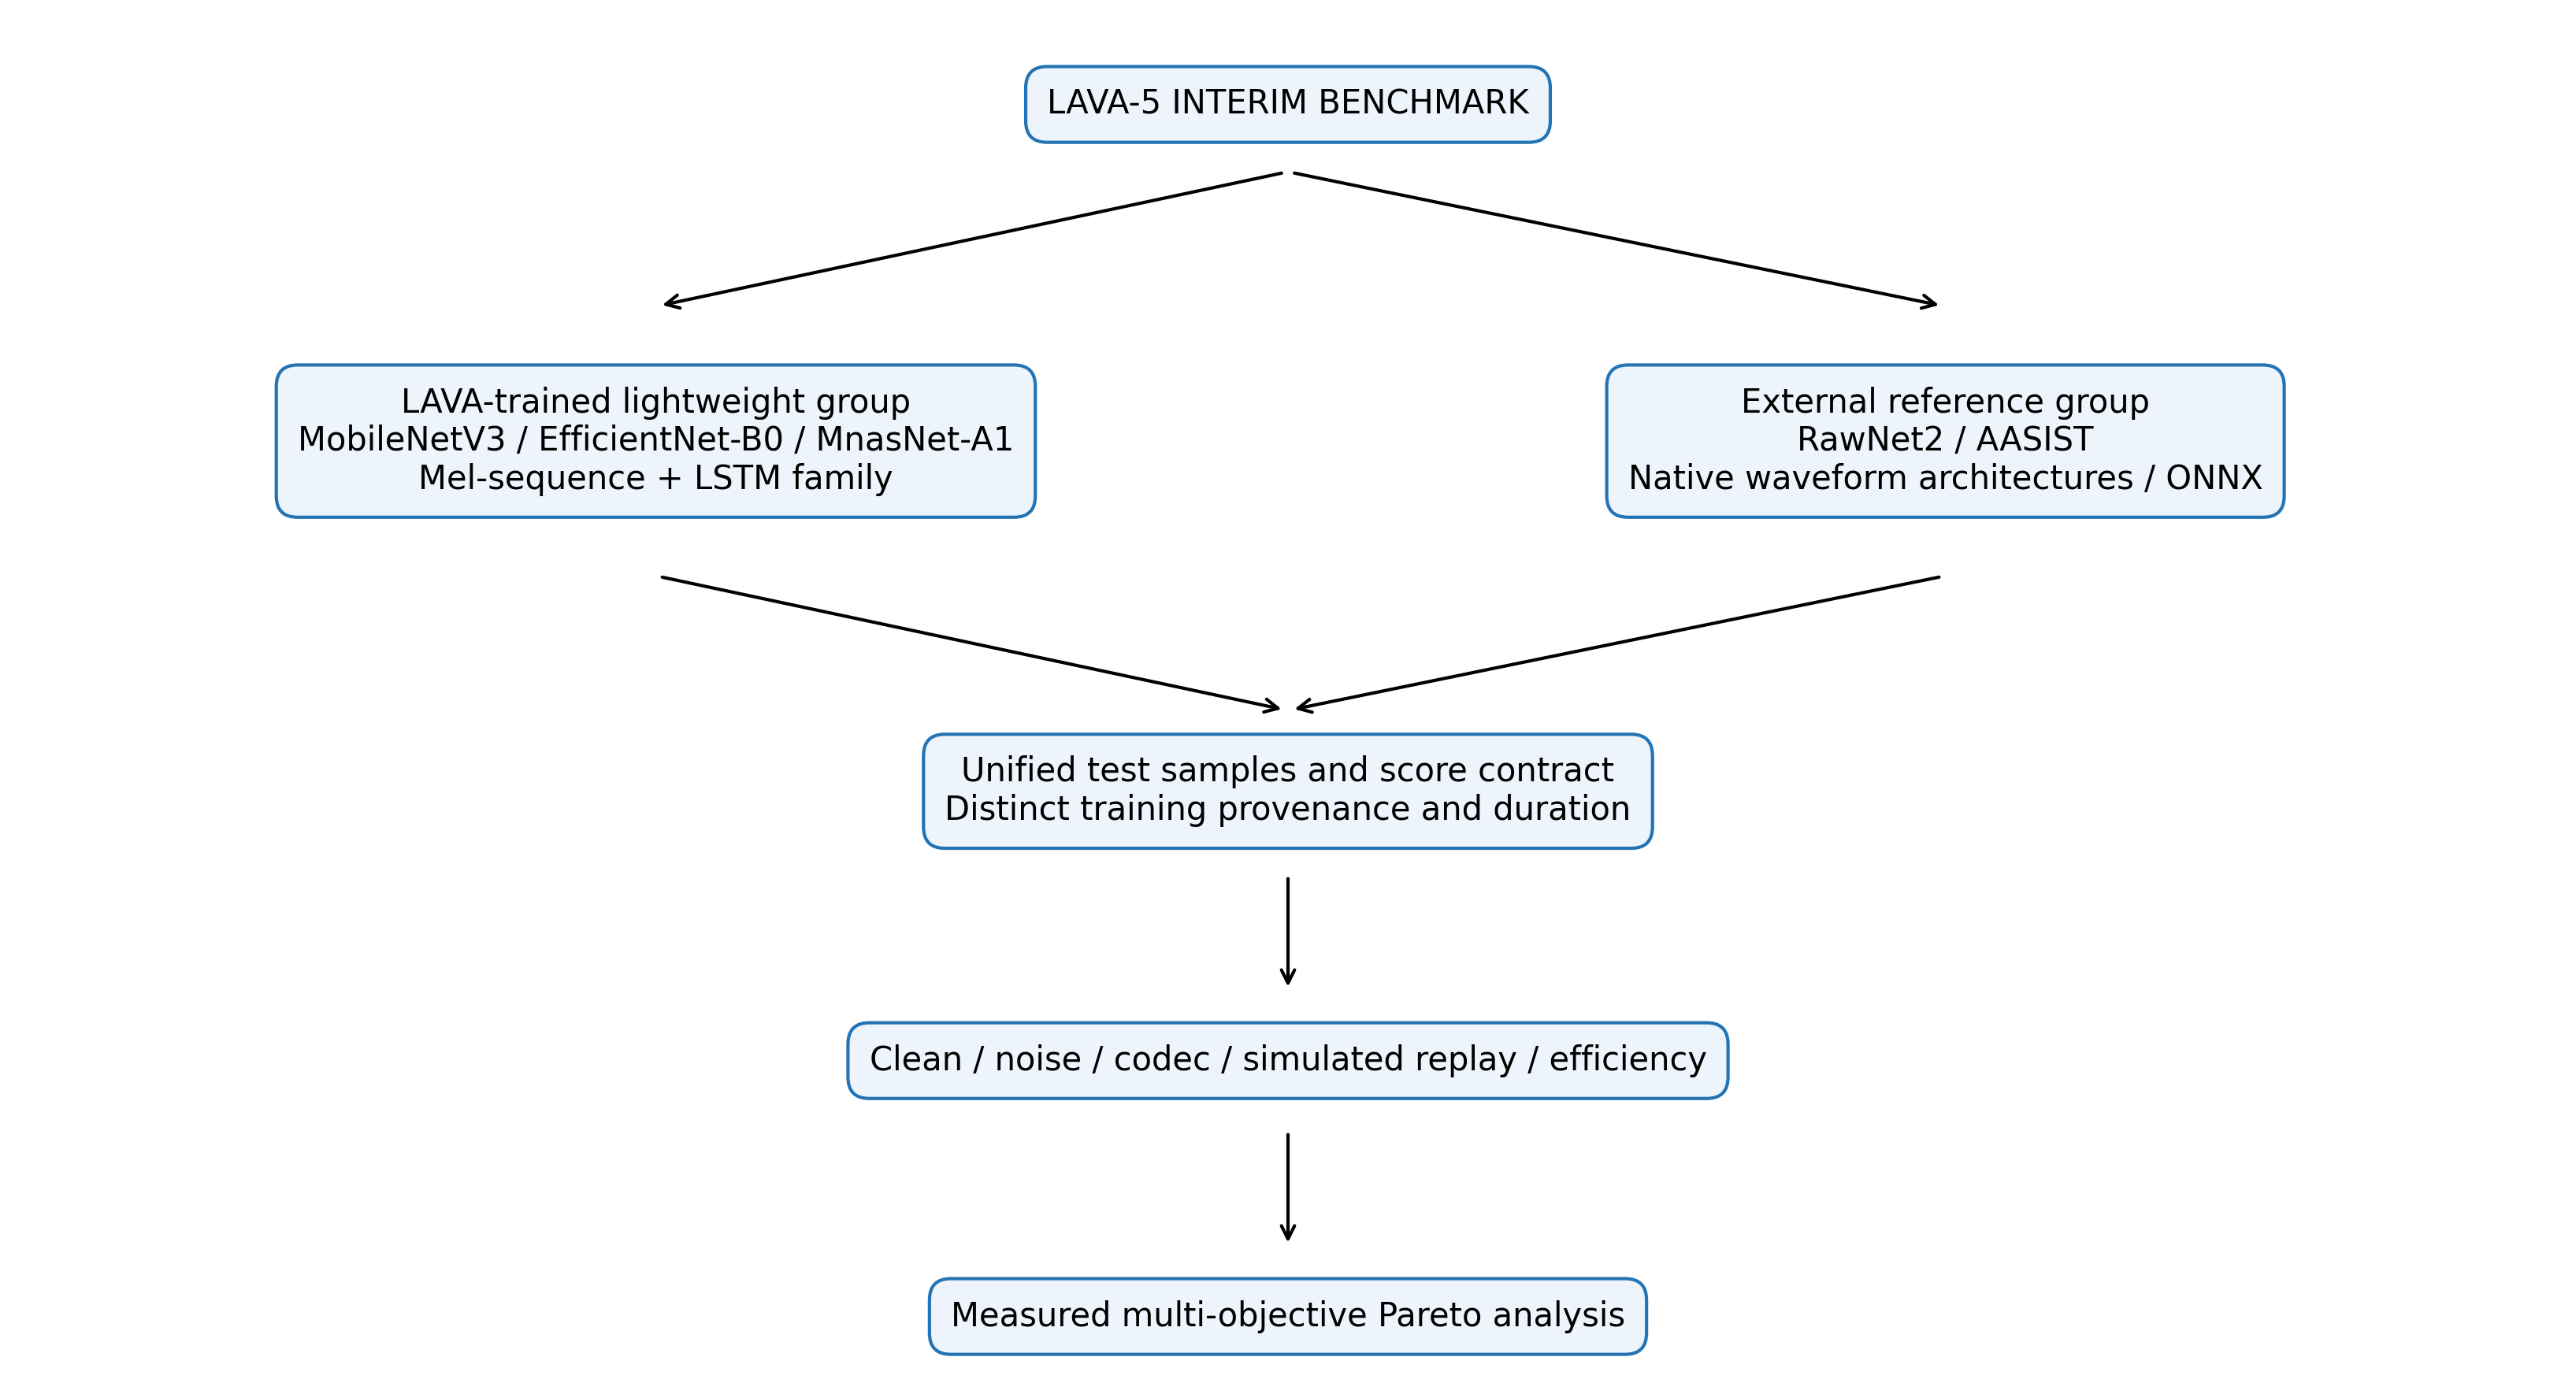
\includegraphics[width=\linewidth]{lava_5_model_overview.png}\caption{LAVA five-detector architecture and evaluation boundary.}\label{fig:overview}\end{figure}
\begin{figure}[t]\centering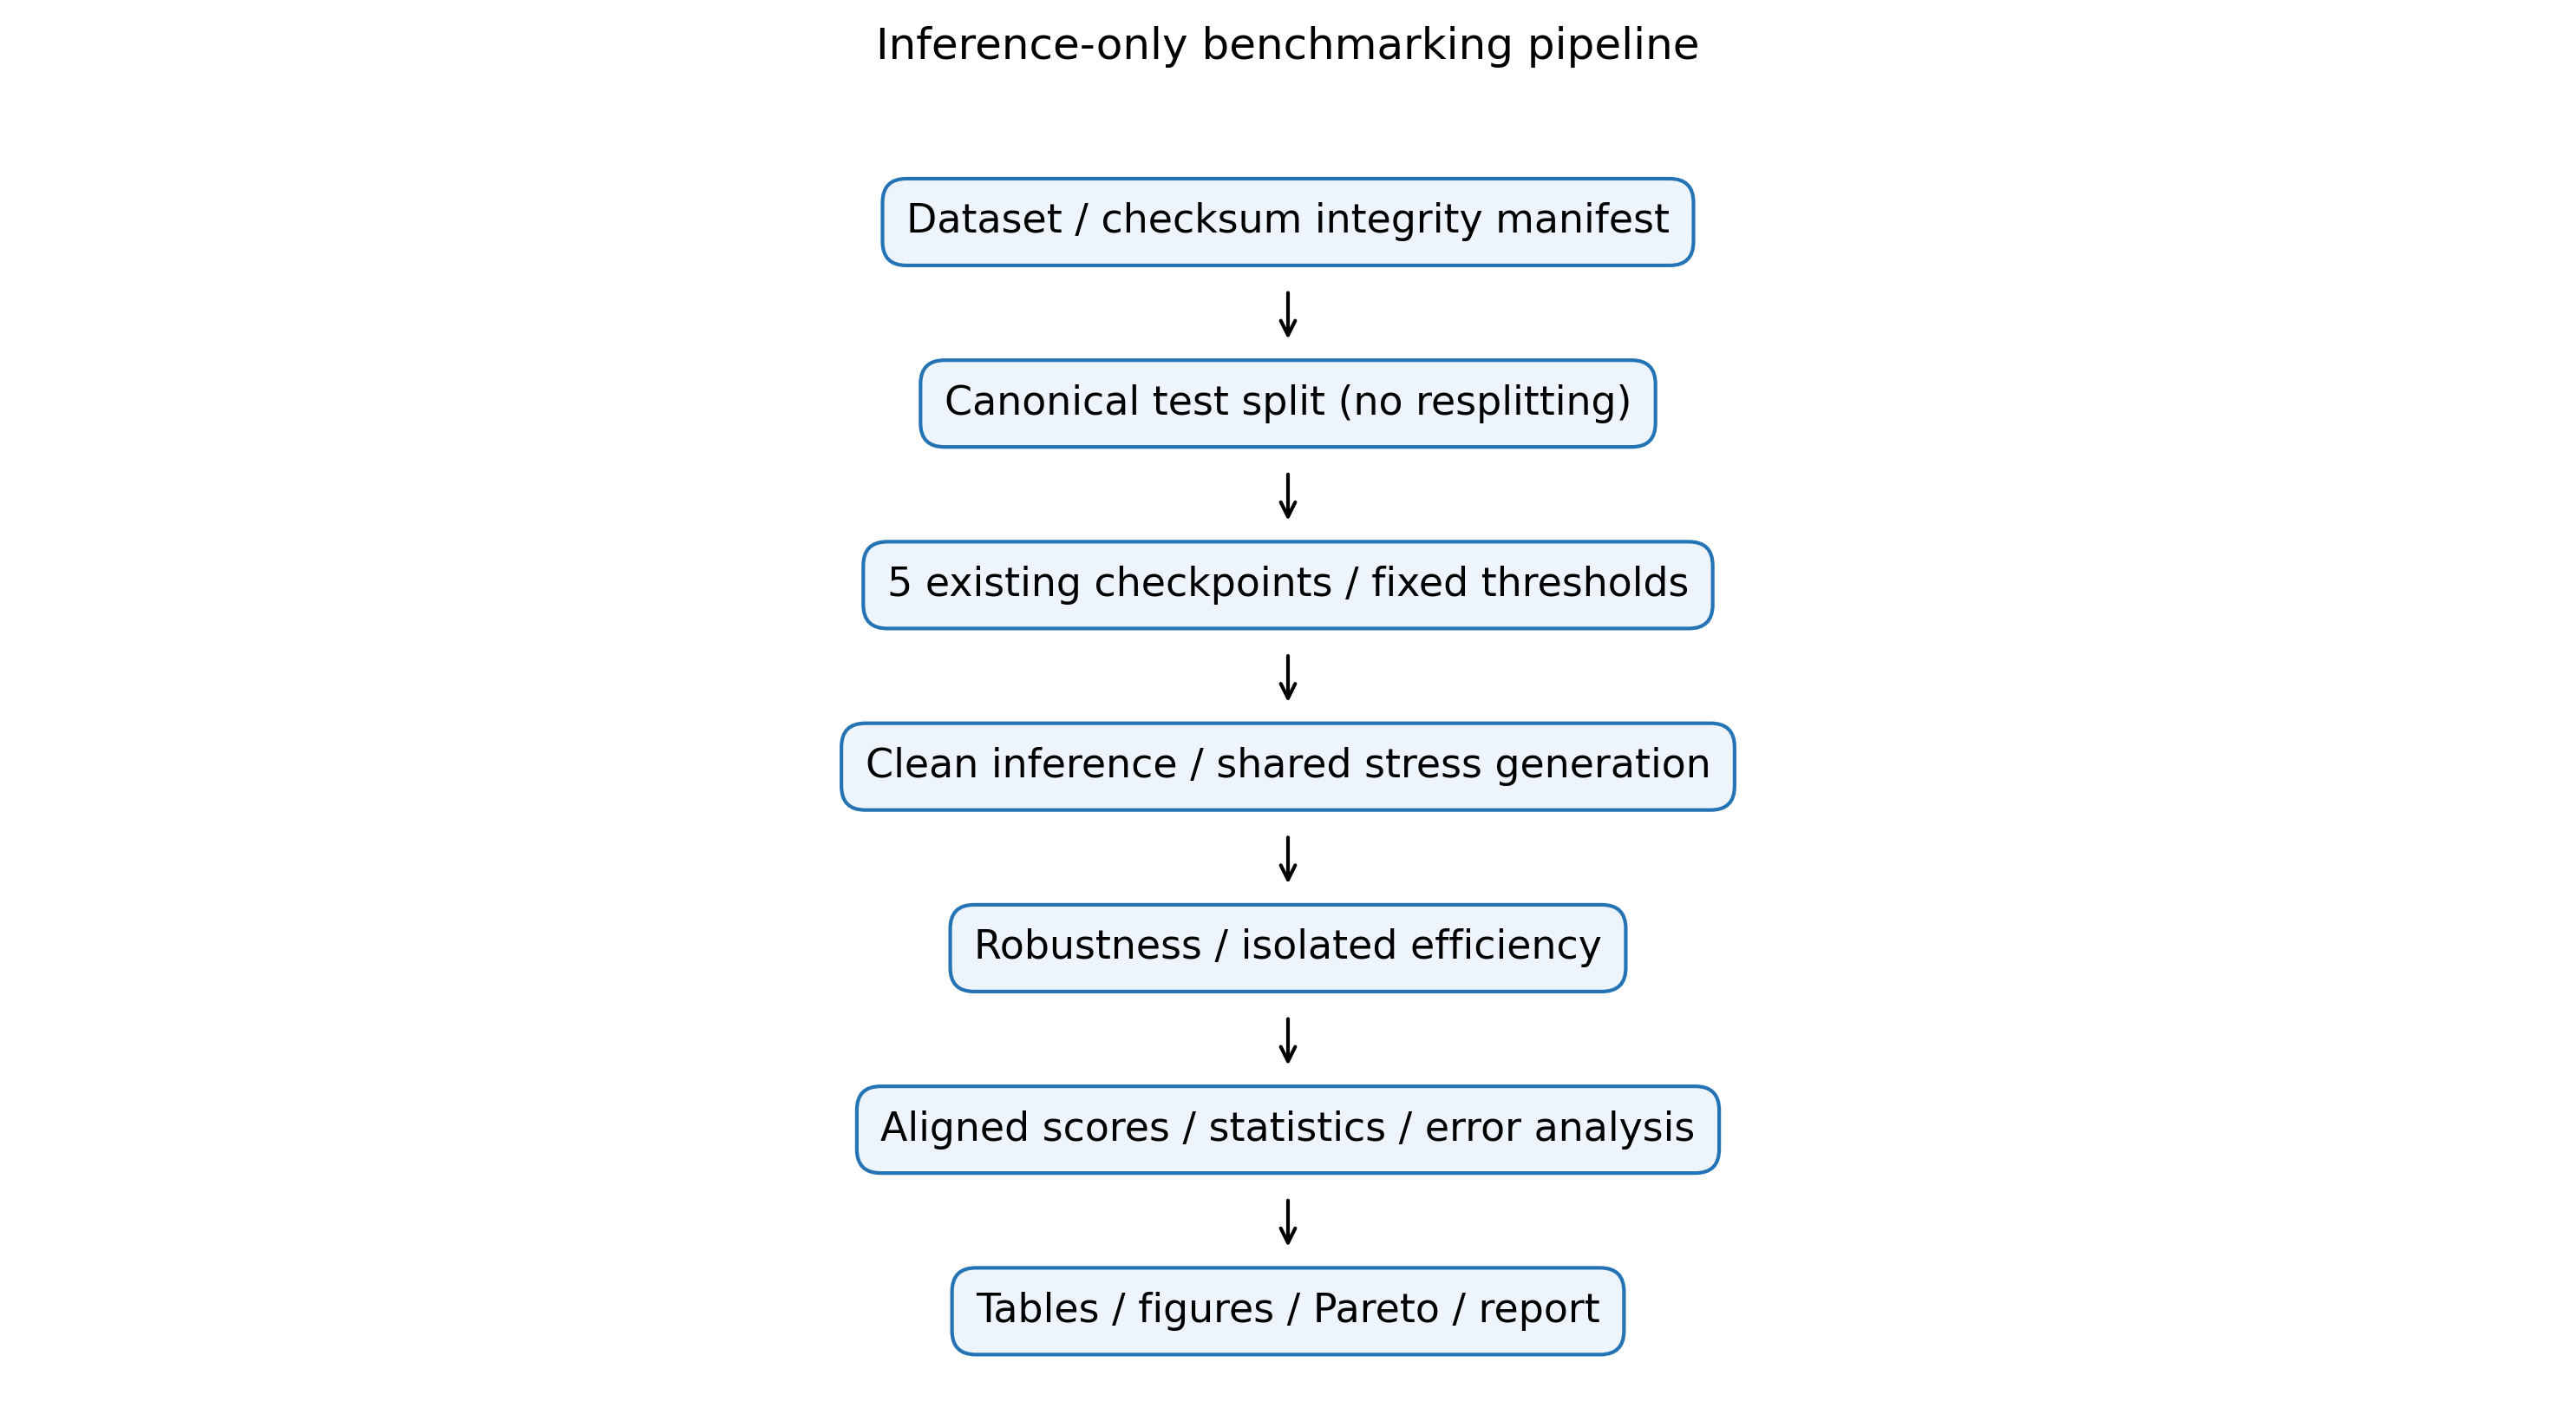
\includegraphics[width=\linewidth]{lava_benchmark_pipeline.png}\caption{Reproducible benchmark pipeline.}\label{fig:pipeline}\end{figure}

The internal dataset has no known speaker, source, generator, parent-recording, or dataset identifiers. Inventory scanned 18,722 files (10,550 REAL; 8,172 FAKE), finding 435 checksum groups, 476 redundant copies, and 14 cross-label groups involving 30 files. Cross-label members were quarantined; one lexicographically first representative was retained per same-label checksum. The final 18,232 samples (10,493 REAL; 7,739 FAKE) were split with seed 42 into 12,762/2,733/2,737 train/validation/test samples. The only supported claim is checksum-group-disjoint. The manifest hash is \texttt{8b55591d...958df9}.

\subsection{Preprocessing and models}
Lightweight audio is converted to mono, polyphase-resampled to 22.05 kHz, zero-padded/truncated to 3 s, and divided chronologically into six 0.5-s segments. Each segment uses a Hann STFT ($n_{fft}=2048$, hop 512), 128 HTK-style Mel bands from 20--8000 Hz, relative-dB clipping at 80 dB, linear [0,255] mapping, bilinear $224\times224$ resizing, and RGB replication. The common head is TimeDistributed(backbone)$\rightarrow$LSTM(128)$\rightarrow$Dense(64, ReLU)$\rightarrow$Dropout(0.4)$\rightarrow$sigmoid.

Reference models consume 64,600 samples at 16 kHz. RawNet2 retains its Sinc/residual/attention/GRU design; AASIST retains Sinc, encoder, graph branches, heterogeneous interaction and readout. Production adapters use polyphase resampling and zero-padding, unlike original librosa/repetition padding. Native--ONNX score parity therefore establishes export fidelity on identical tensors, not paper-pipeline equivalence.

Table~\ref{tab:detectors} summarizes the evaluated artifacts and preserves the distinction between locally trained lightweight models and externally pretrained references.

\begin{table*}[t]\caption{Detector configuration and provenance.}\label{tab:detectors}\centering\small
\begin{tabularx}{\textwidth}{l l l l X r X}\toprule Model&Group&Runtime&Input&Mechanism&Params&Provenance\\\midrule
MobileNetV3-LSTM&Light&TF 2.15&Mel, 3 s&576-D backbone + LSTM&1,308,401&LAVA, ImageNet\\
EfficientNet-B0-LSTM&Light&TF 2.15&Mel, 3 s&1280-D backbone + LSTM&4,779,300&LAVA, ImageNet, warm-up best\\
MnasNet-A1-LSTM&Light&TF 2.15&Mel, 3 s&1280-D backbone + LSTM&3,369,255&LAVA, scratch, early-stopped best\\
RawNet2&Reference&ONNX/PyTorch&Wave, 4.0375 s&Sinc/residual/attention/GRU&17,621,410&External checkpoint\\
AASIST&Reference&ONNX/PyTorch&Wave, 4.0375 s&Heterogeneous graph attention&297,866&External checkpoint\\\bottomrule
\end{tabularx}\end{table*}

\subsection{Training and scores}
MobileNet used ImageNet initialization, frozen-backbone warm-up and partial low-rate fine-tuning with frozen BatchNorm. EfficientNet is the best available warm-up checkpoint (epoch 47, validation loss 0.1698), not a completed fine-tune lifecycle. MnasNet was scratch-trained end-to-end; the deployed best is epoch 27 from a 39-epoch early-stopped run, using Adam $10^{-4}$, clip norm 1, label smoothing 0.1 and L2 coefficient $10^{-5}$. RawNet2/AASIST were not LAVA-trained. Six-tensor native--ONNX maximum score differences were $4.11\times10^{-6}$ and $5.96\times10^{-8}$.

REAL=0, FAKE=1, and all adapters expose $p=\pfake$:
\begin{equation}\hat y=\begin{cases}1&p\ge\tau\\0&p<\tau.\end{cases}\label{eq:decision}\end{equation}
Validation-F1 thresholds are 0.82/0.90/0.90 for MobileNet/EfficientNet/MnasNet. References retain uncalibrated 0.5 defaults. Test labels select neither weights nor thresholds.

\subsection{Metrics, stress, and timing}
\begin{align}P&=TP/(TP+FP),\quad R=TP/(TP+FN),\nonumber\\F1&=2PR/(P+R).\label{eq:f1}\end{align}
ROC-AUC uses raw $p$. With $FAR=FP/(FP+TN)$ and $FRR=FN/(FN+TP)$, EER is linearly interpolated where $FAR\simeq FRR$ and reported as their mean.

Robustness uses a prediction-independent stratified subset of 100 test samples (58 REAL; 42 FAKE; seed 42). Conditions are seeded AWGN at 20/10/5/0 dB; FFmpeg MP3 128/64, Opus 64, and AAC 96 kb/s round trips; and one simulated channel with 0/17/43/89-ms taps plus fourth-order 100--3800-Hz band-pass. Replay is not physical. For each condition, $\Delta F1=F1_{clean}-F1_{stress}$; the overall value is the arithmetic mean across nine conditions.

Efficiency uses sequential isolated CPU processes, float32, batch one, one computational thread, ten warm-ups and 50 timed runs. Startup/tracing are excluded. RSS is whole-process sampled memory. 
\begin{equation}RTF=T_{processing}/T_{audio},\quad \mathrm{Throughput}=N/T_{total}.\label{eq:rtf}\end{equation}
RTF below one means faster-than-duration offline inference, not causal streaming.

The diagnostic Pareto objectives minimize subset EER, mean $\Delta F1$, and RTF. $A$ dominates $B$ iff
\begin{equation}f_i(A)\le f_i(B)\ \forall i,\quad \exists j:f_j(A)<f_j(B).\label{eq:pareto}\end{equation}
No weighted score is used. Uncertainty uses 1,000 shared stratified test bootstraps; it is not multi-seed uncertainty.

\section{Results}
\subsection{Clean performance (RQ1)}
All five artifacts passed load, score-bound, hash, and adapter-parity checks. Table~\ref{tab:clean} and Figs.~\ref{fig:roc}--\ref{fig:det} use all 2,737 test samples.
\begin{table*}[t]\caption{Full canonical-test clean performance.}\label{tab:clean}\centering\small
\begin{tabular}{lrrrrrrrrl}\toprule Model&Acc.&Prec.&Rec.&F1&Macro-F1&AUC&EER& &TN/FP/FN/TP\\\midrule
MobileNet&.9766&.9741&.9707&.9724&.9761&.9911&.0250&&1545/30/34/1128\\
EfficientNet&.9635&.9724&.9406&.9563&.9624&.9877&.0400&&1544/31/69/1093\\
MnasNet&.9697&.9599&.9690&.9645&.9690&.9886&.0310&&1528/47/36/1126\\
RawNet2 ext.&.4936&.4380&.6807&.5330&.4900&.5178&.4813&&560/1015/371/791\\
AASIST ext.&.5513&.4758&.5585&.5139&.5487&.5597&.4463&&860/715/513/649\\\bottomrule
\end{tabular}\end{table*}
\begin{figure}[t]\centering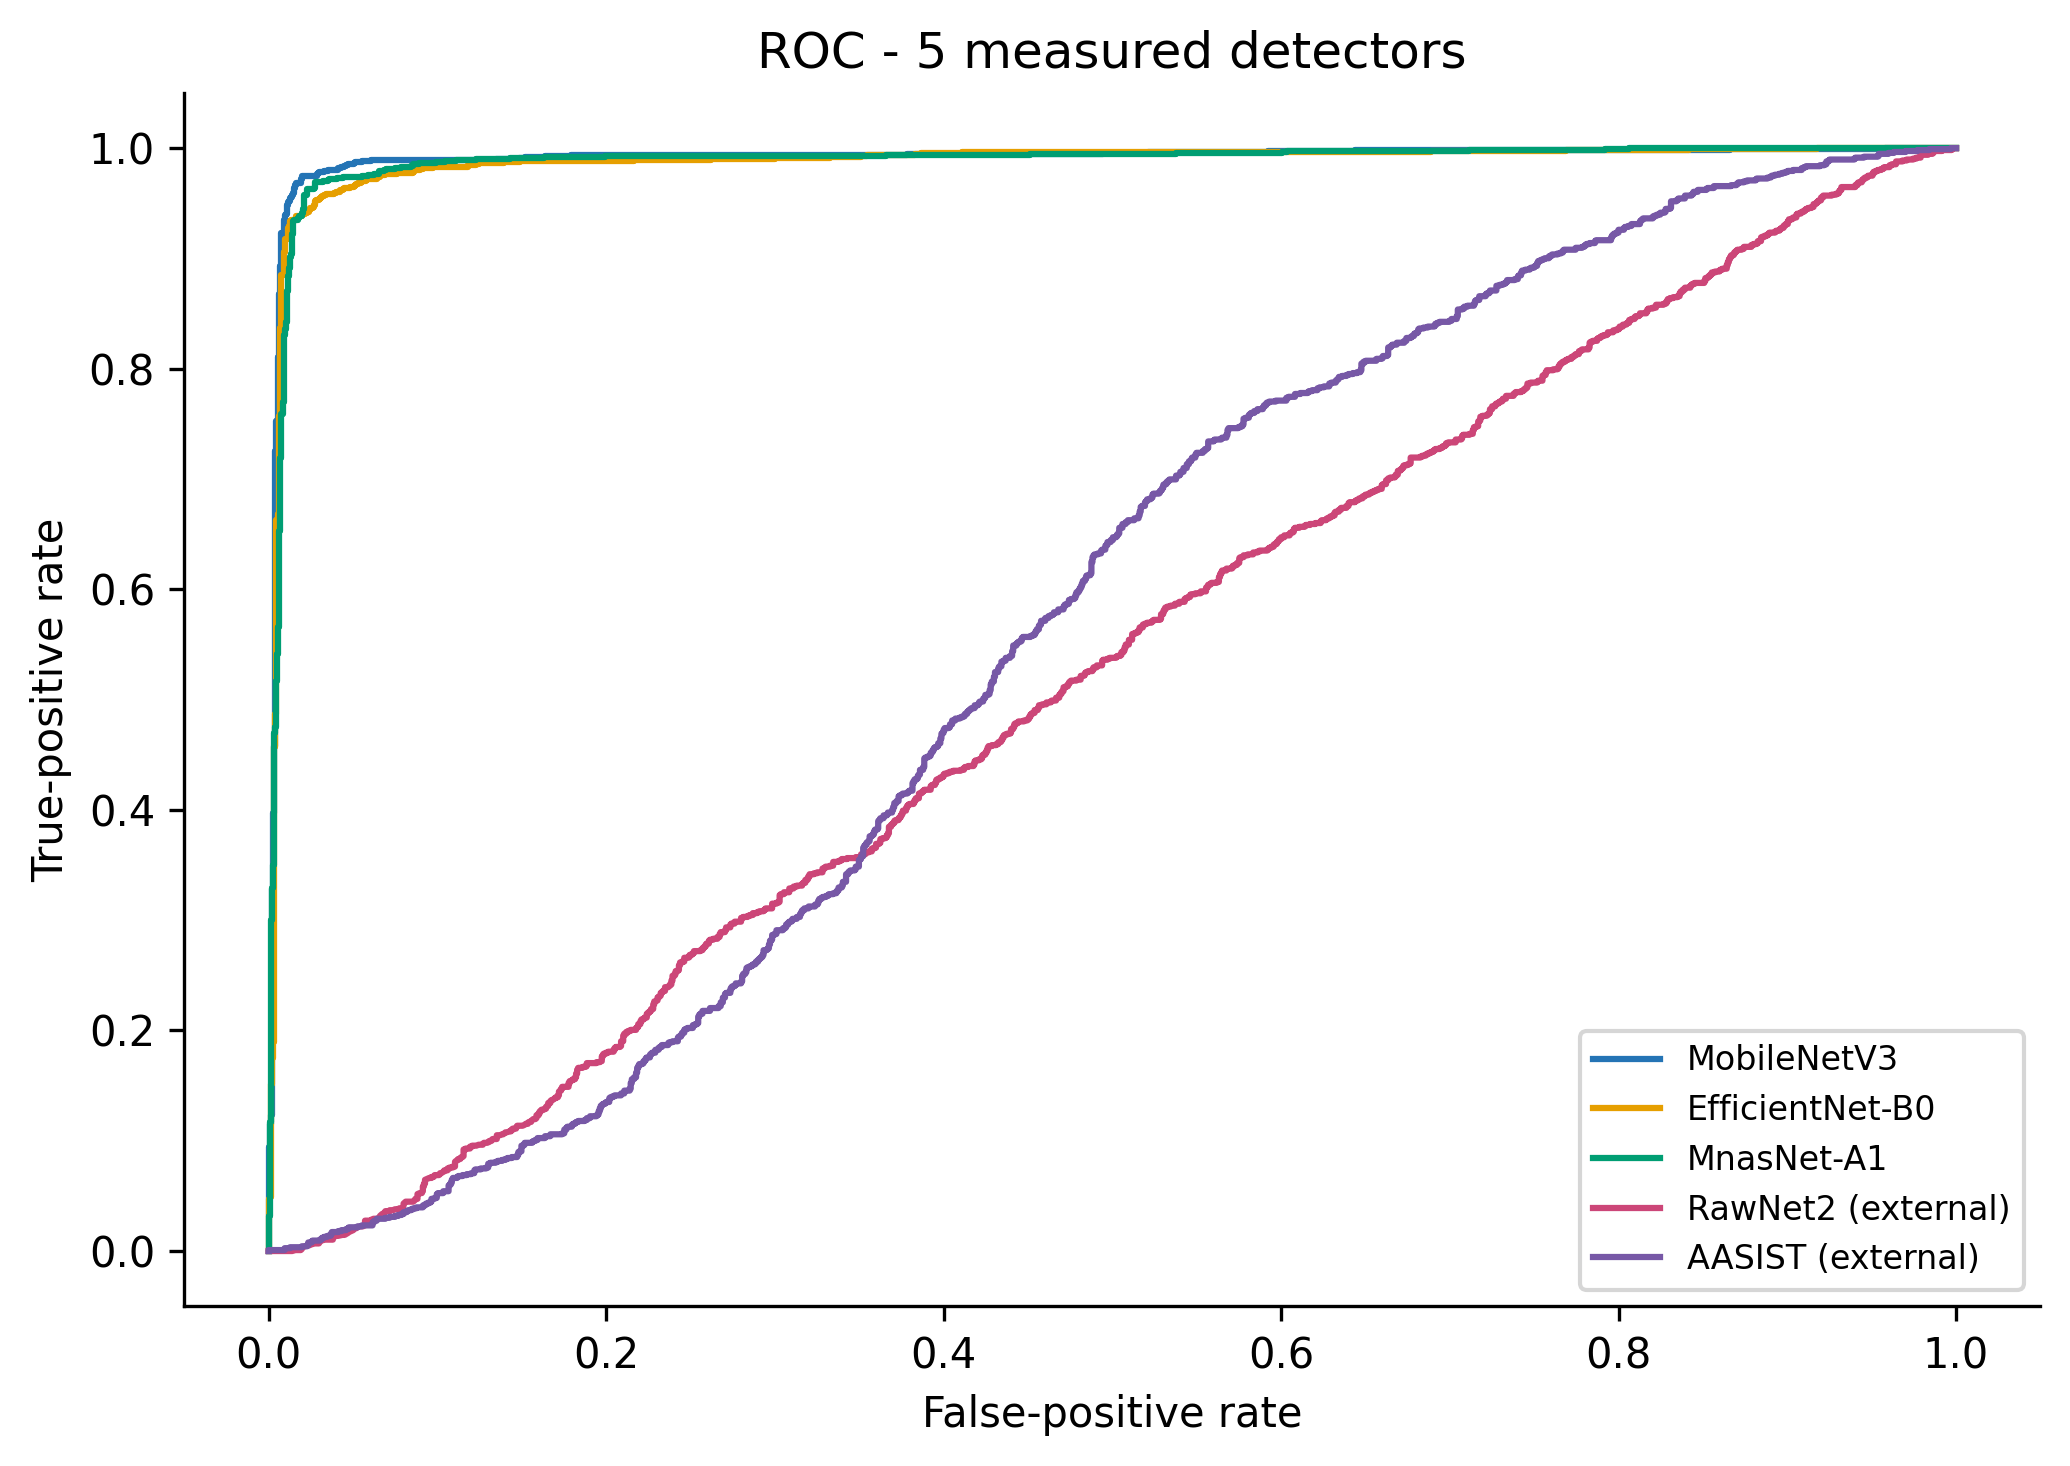
\includegraphics[width=\linewidth]{roc_comparison_5_models.png}\caption{Full-test ROC curves.}\label{fig:roc}\end{figure}
\begin{figure}[t]\centering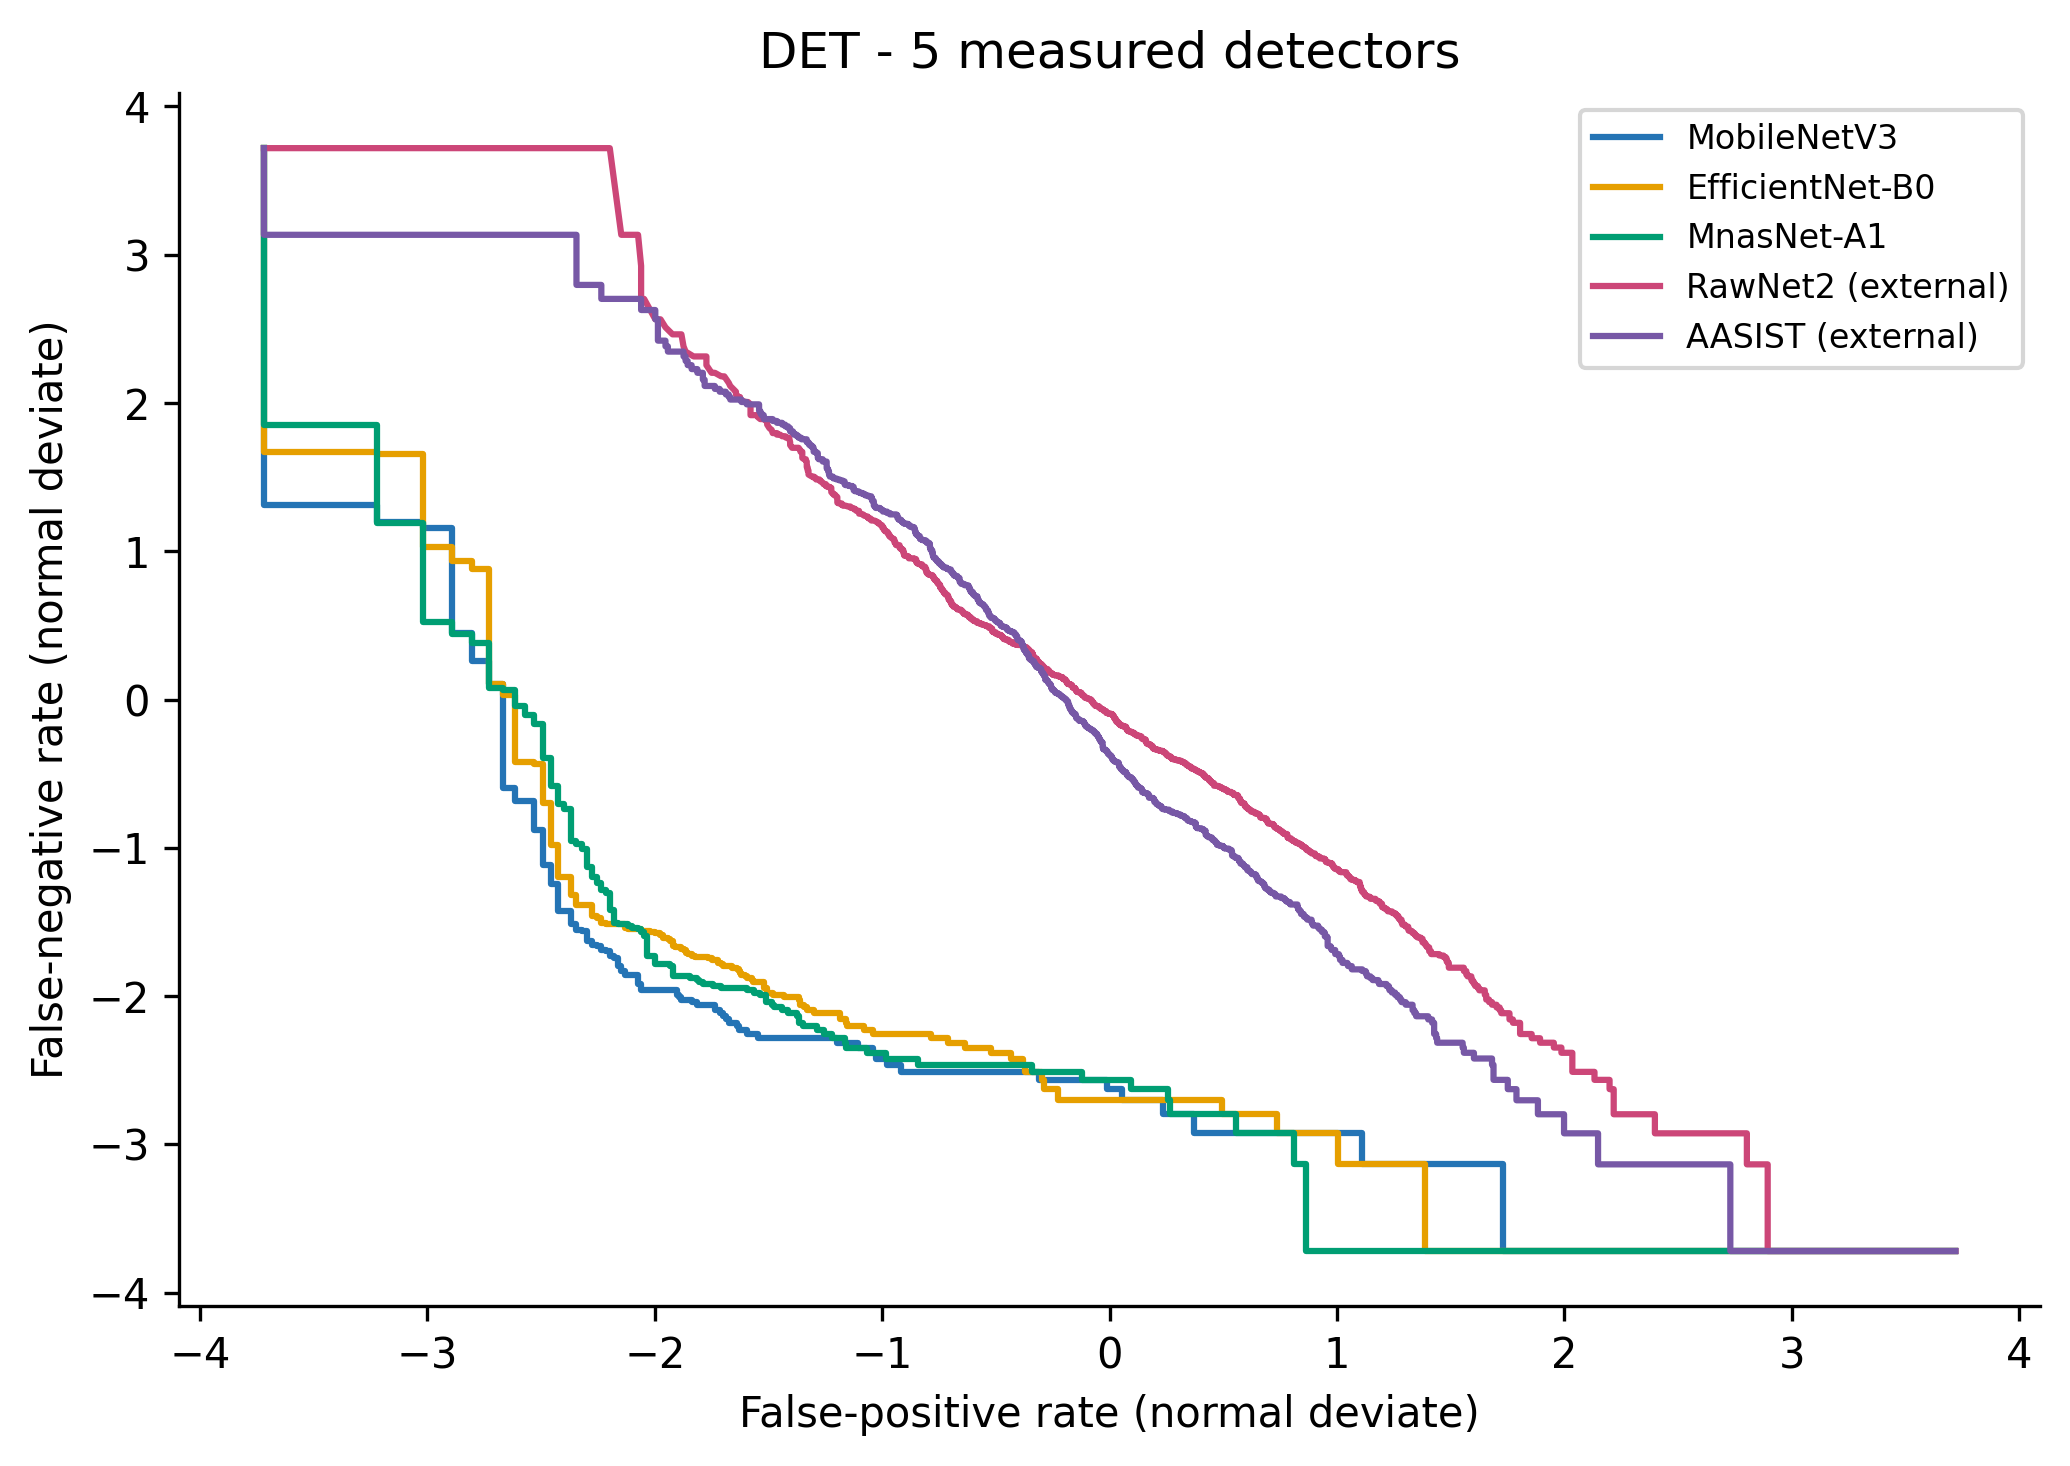
\includegraphics[width=\linewidth]{det_comparison_5_models.png}\caption{Full-test DET curves.}\label{fig:det}\end{figure}
The three local lightweight artifacts exceed the external references under this specific contract. MobileNet leads clean aggregates. Different provenance, durations, thresholds and preprocessing prohibit an architecture-only ranking.

\subsection{Diagnostic robustness (RQ2)}
Table~\ref{tab:robust} reports mean diagnostic degradation by stress family.
\begin{table}[t]\caption{Mean diagnostic $\Delta F1$ (lower is better).}\label{tab:robust}\centering\small
\begin{tabular}{lrrrr}\toprule Model&Noise&Codec&Replay&All 9\\\midrule MobileNet&.6722&.0095&.0620&.3099\\EfficientNet&.8053&.0000&.0641&.3650\\MnasNet&.6119&.0233&.1489&.2989\\RawNet2&.5077&-.0007&-.0109&.2241\\AASIST&-.0660&-.0074&-.0682&-.0402\\\bottomrule\end{tabular}\end{table}
Codec changes were small for lightweight models, whereas AWGN was damaging (Figs.~\ref{fig:noise} and~\ref{fig:heat}). Simulated replay F1 was 0.9136/0.8989/0.8267 for MobileNet/EfficientNet/MnasNet. Negative degradation for weak reference baselines is not evidence of superior robustness.
\begin{figure}[t]\centering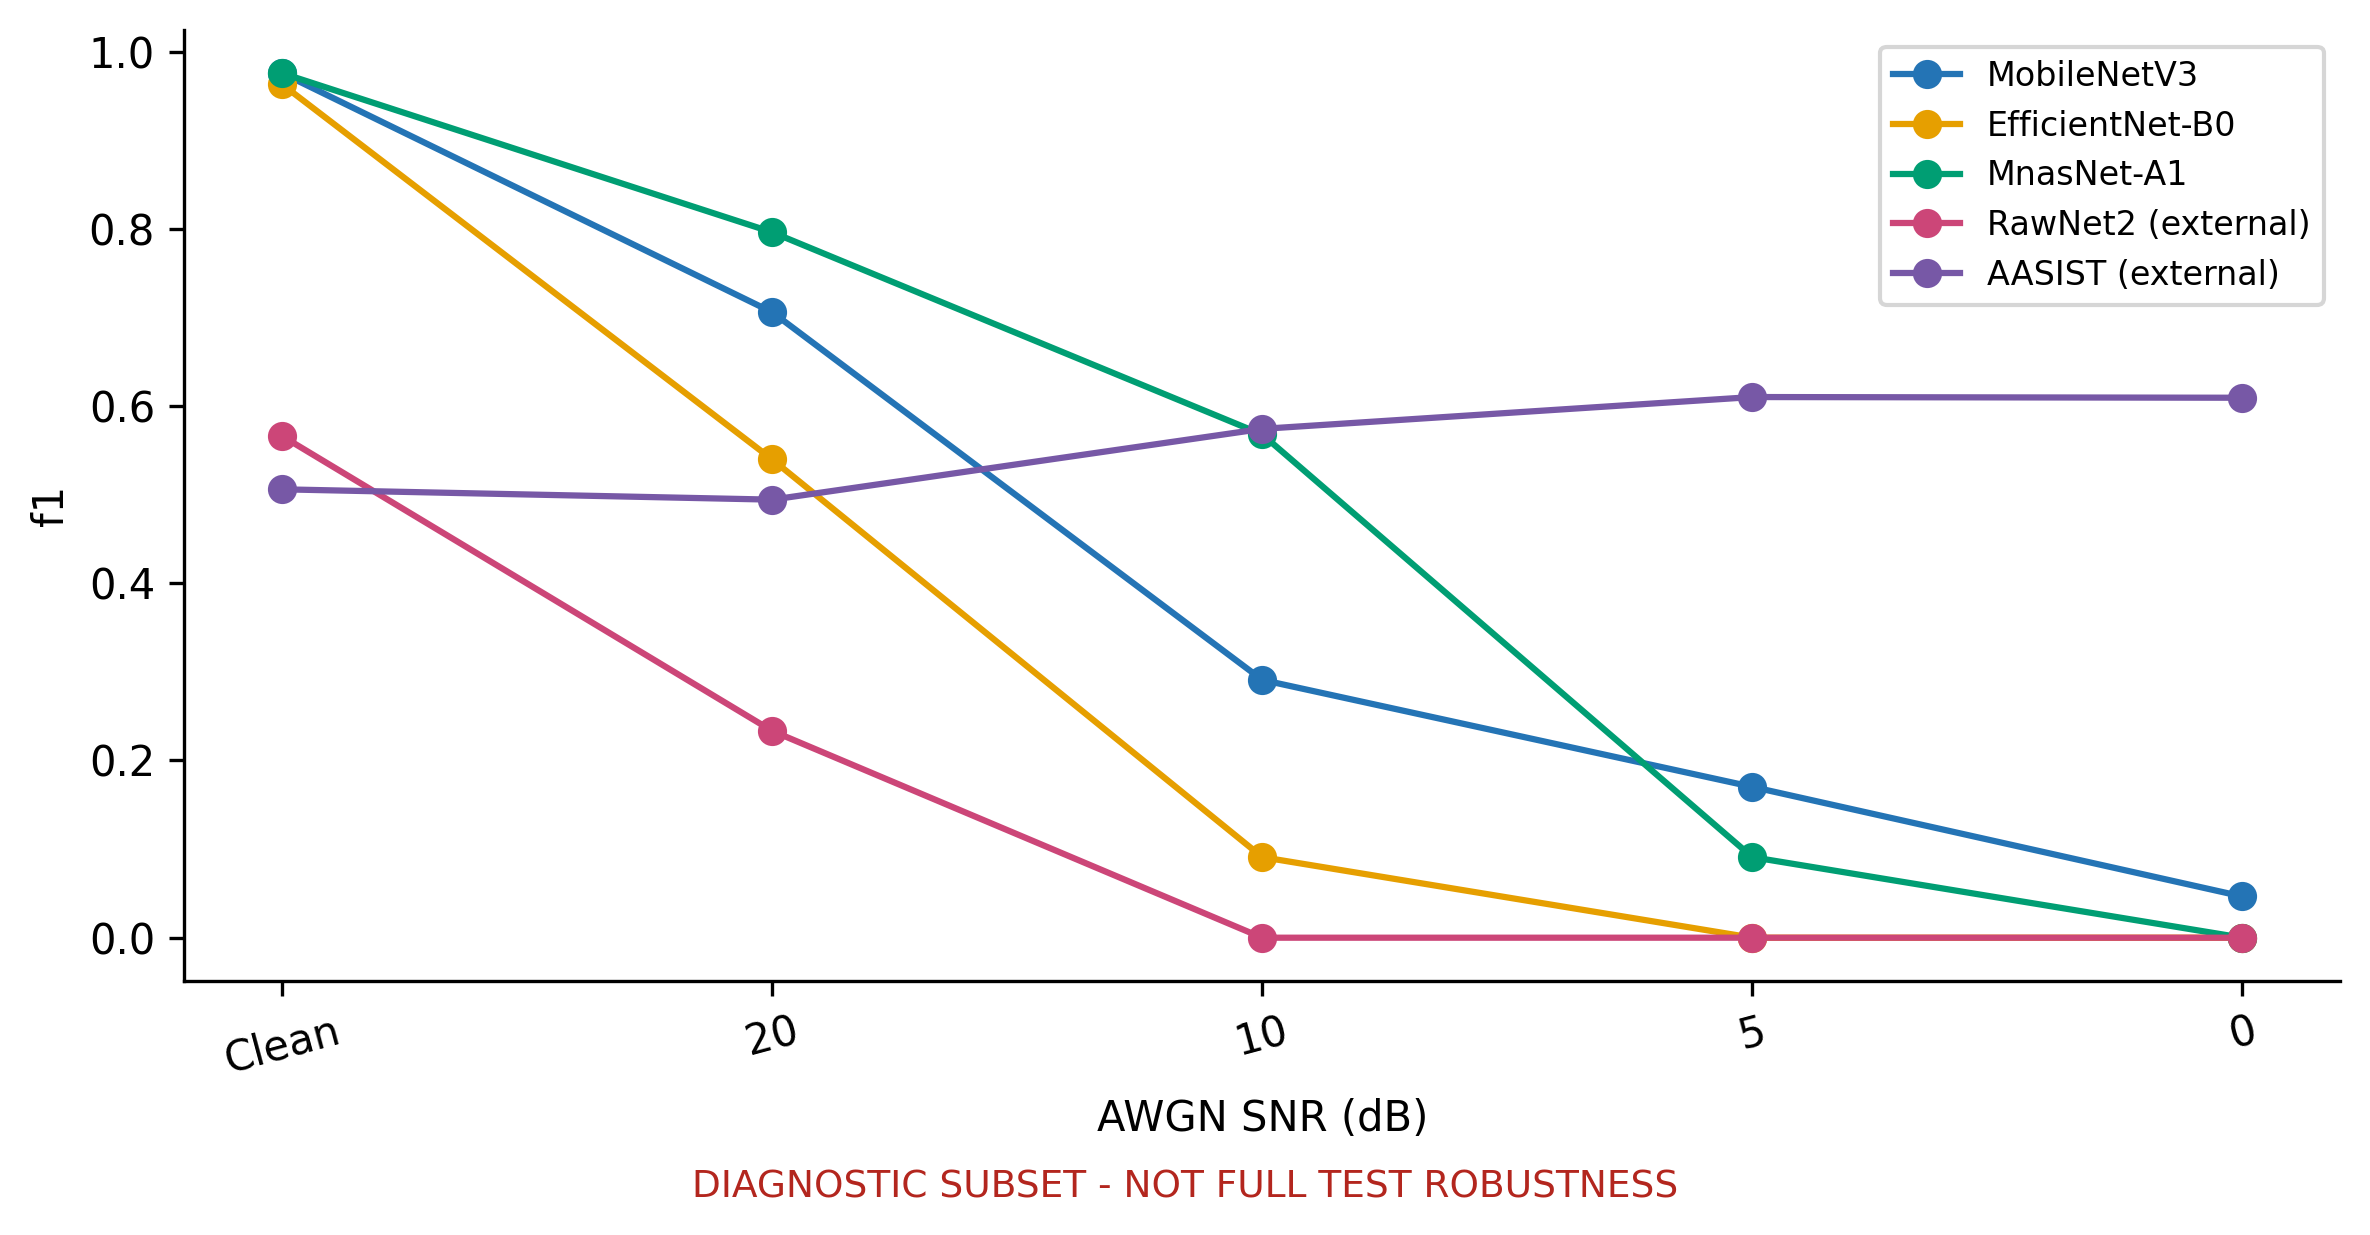
\includegraphics[width=\linewidth]{noise_f1_vs_snr.png}\caption{Diagnostic F1 under AWGN; not full-test robustness.}\label{fig:noise}\end{figure}
\begin{figure}[t]\centering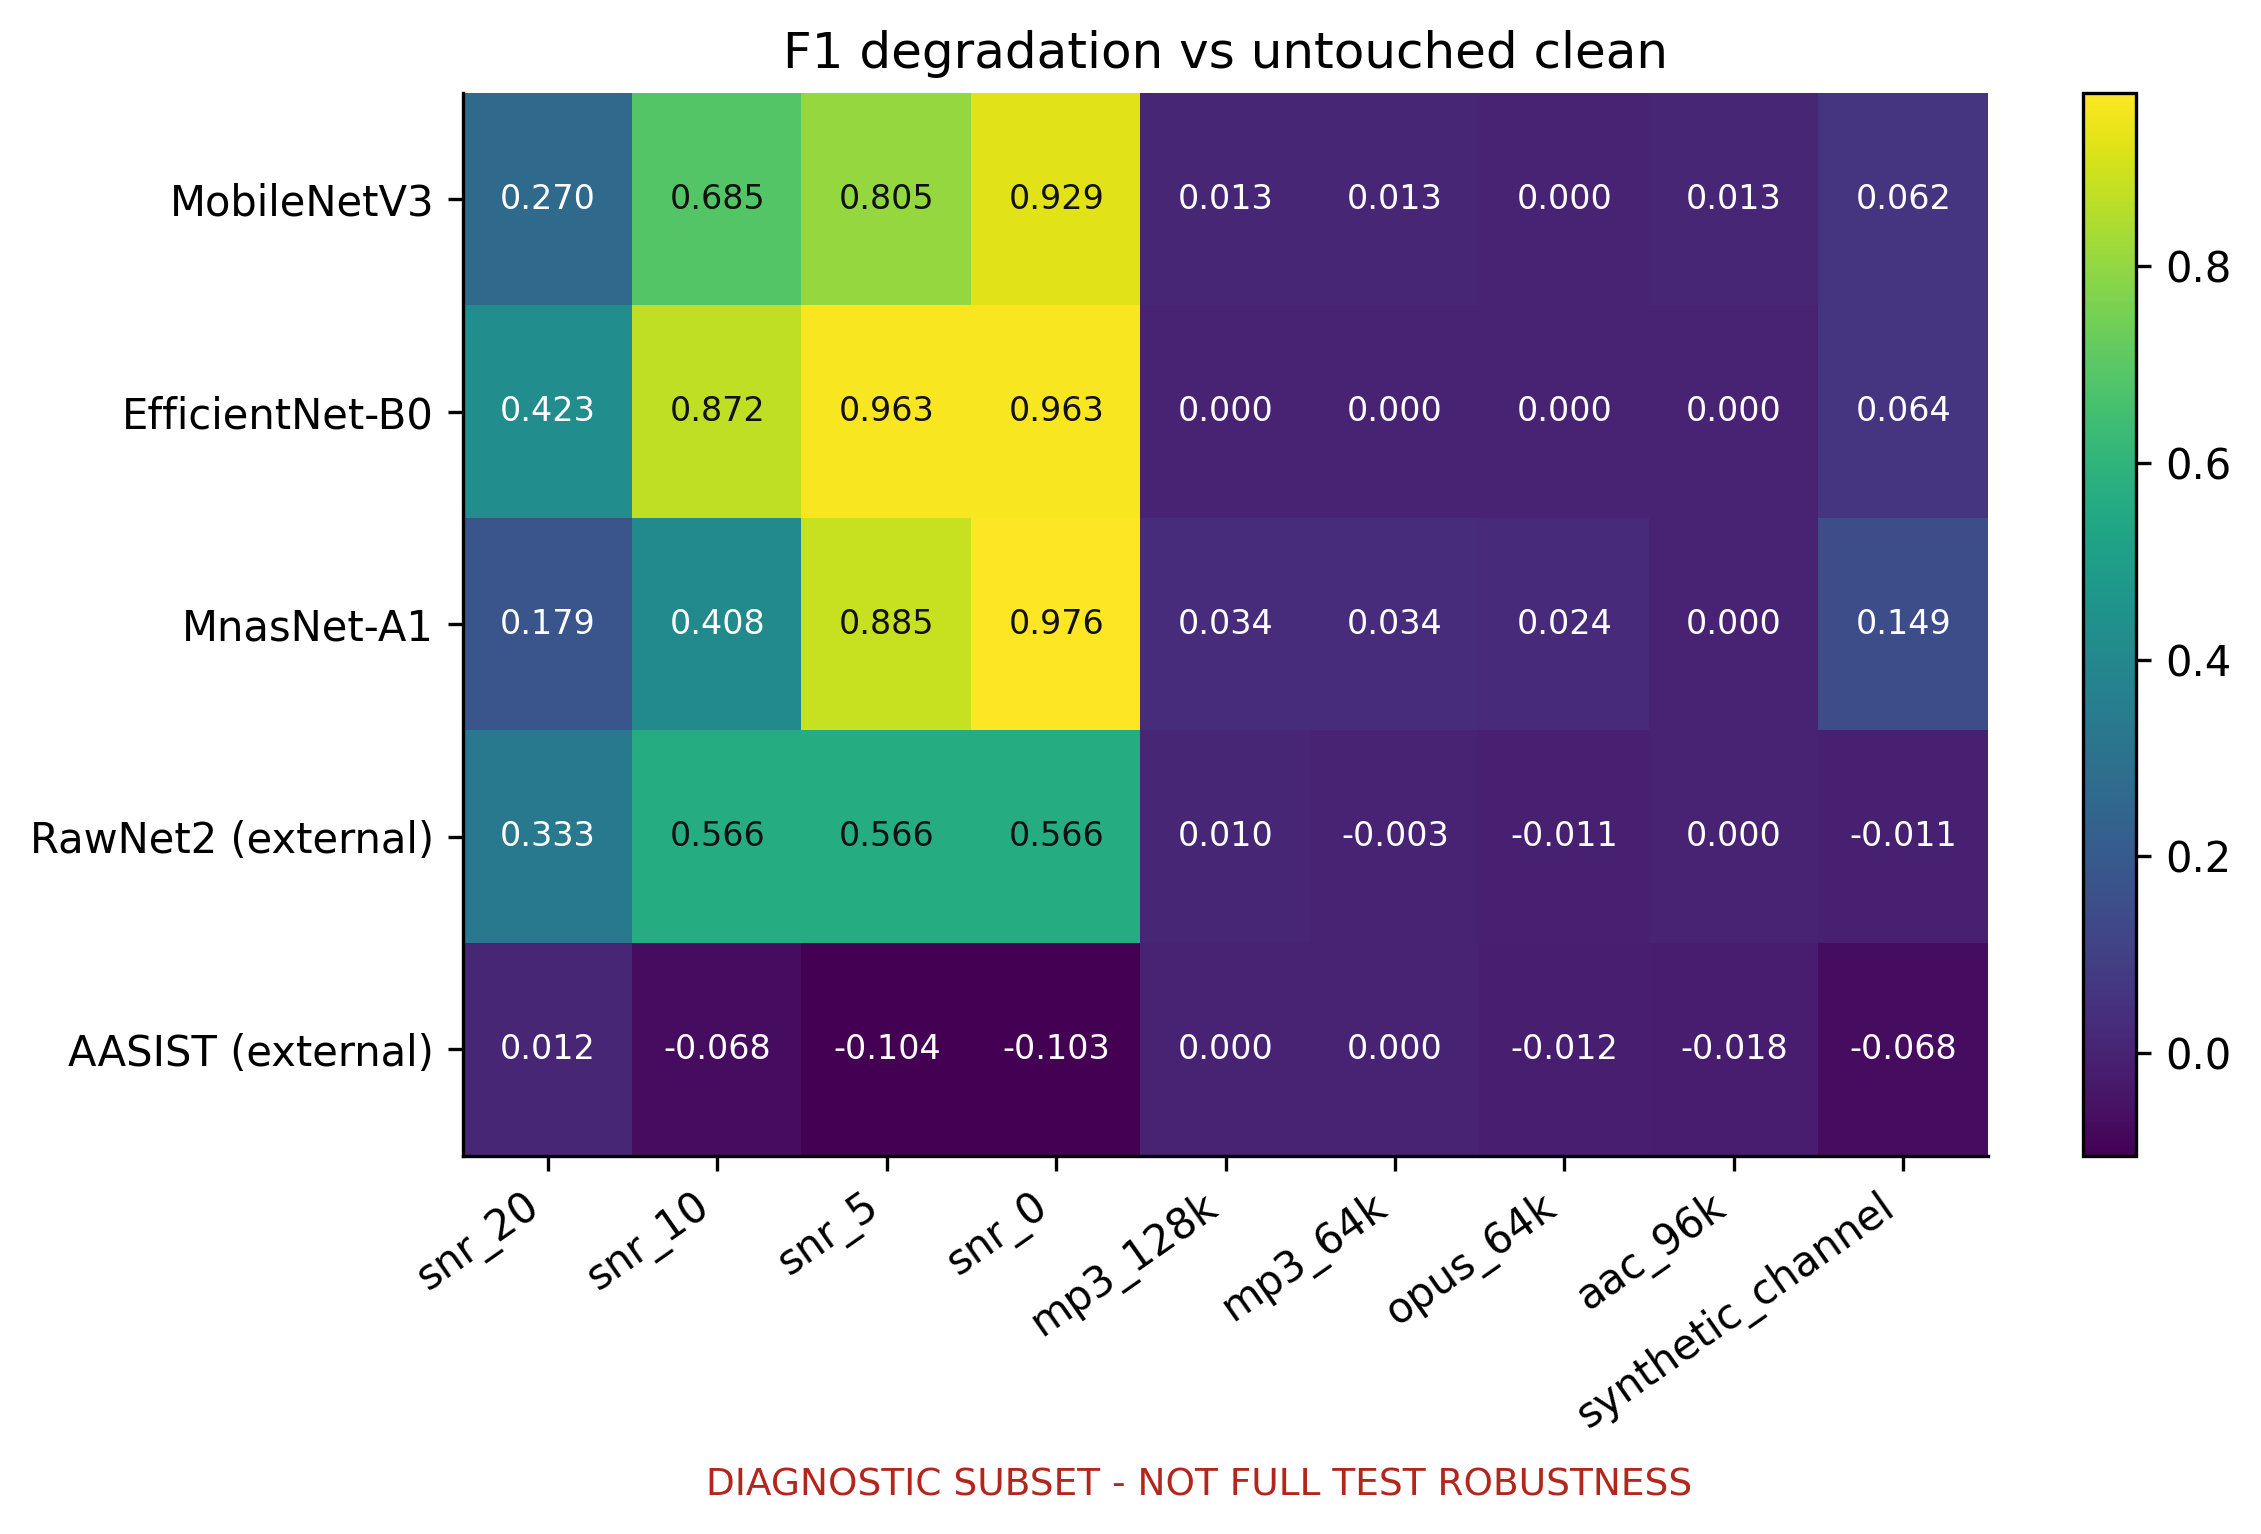
\includegraphics[width=\linewidth]{robustness_heatmap.png}\caption{Per-condition diagnostic $\Delta F1$.}\label{fig:heat}\end{figure}

\subsection{Efficiency}
Table~\ref{tab:eff} reports the measured efficiency quantities.
\begin{table*}[t]\caption{Single-thread desktop-CPU efficiency.}\label{tab:eff}\centering\small
\begin{tabular}{lrrrrrrrr}\toprule Model&Size MiB&RSS MiB&Pre ms&Model ms&Mean/P95 ms&clips/s&RTF\\\midrule
MobileNet&5.64&554.6&13.43&30.07&43.81/52.12&22.83&.0146\\EfficientNet&18.96&651.2&13.59&168.36&175.85/196.11&5.69&.0586\\MnasNet&13.43&566.0&13.60&95.25&117.00/138.96&8.55&.0390\\RawNet2&67.65&249.5&.63&95.10&96.54/102.62&10.36&.0239\\AASIST&1.61&442.5&.47&359.61&362.91/398.45&2.76&.0899\\\bottomrule\end{tabular}\end{table*}
MobileNet is fastest; AASIST is smallest but slowest, showing that size alone does not predict runtime. All results are desktop CPU evidence, not edge validation (Figs.~\ref{fig:lat} and~\ref{fig:params}).
\begin{figure}[t]\centering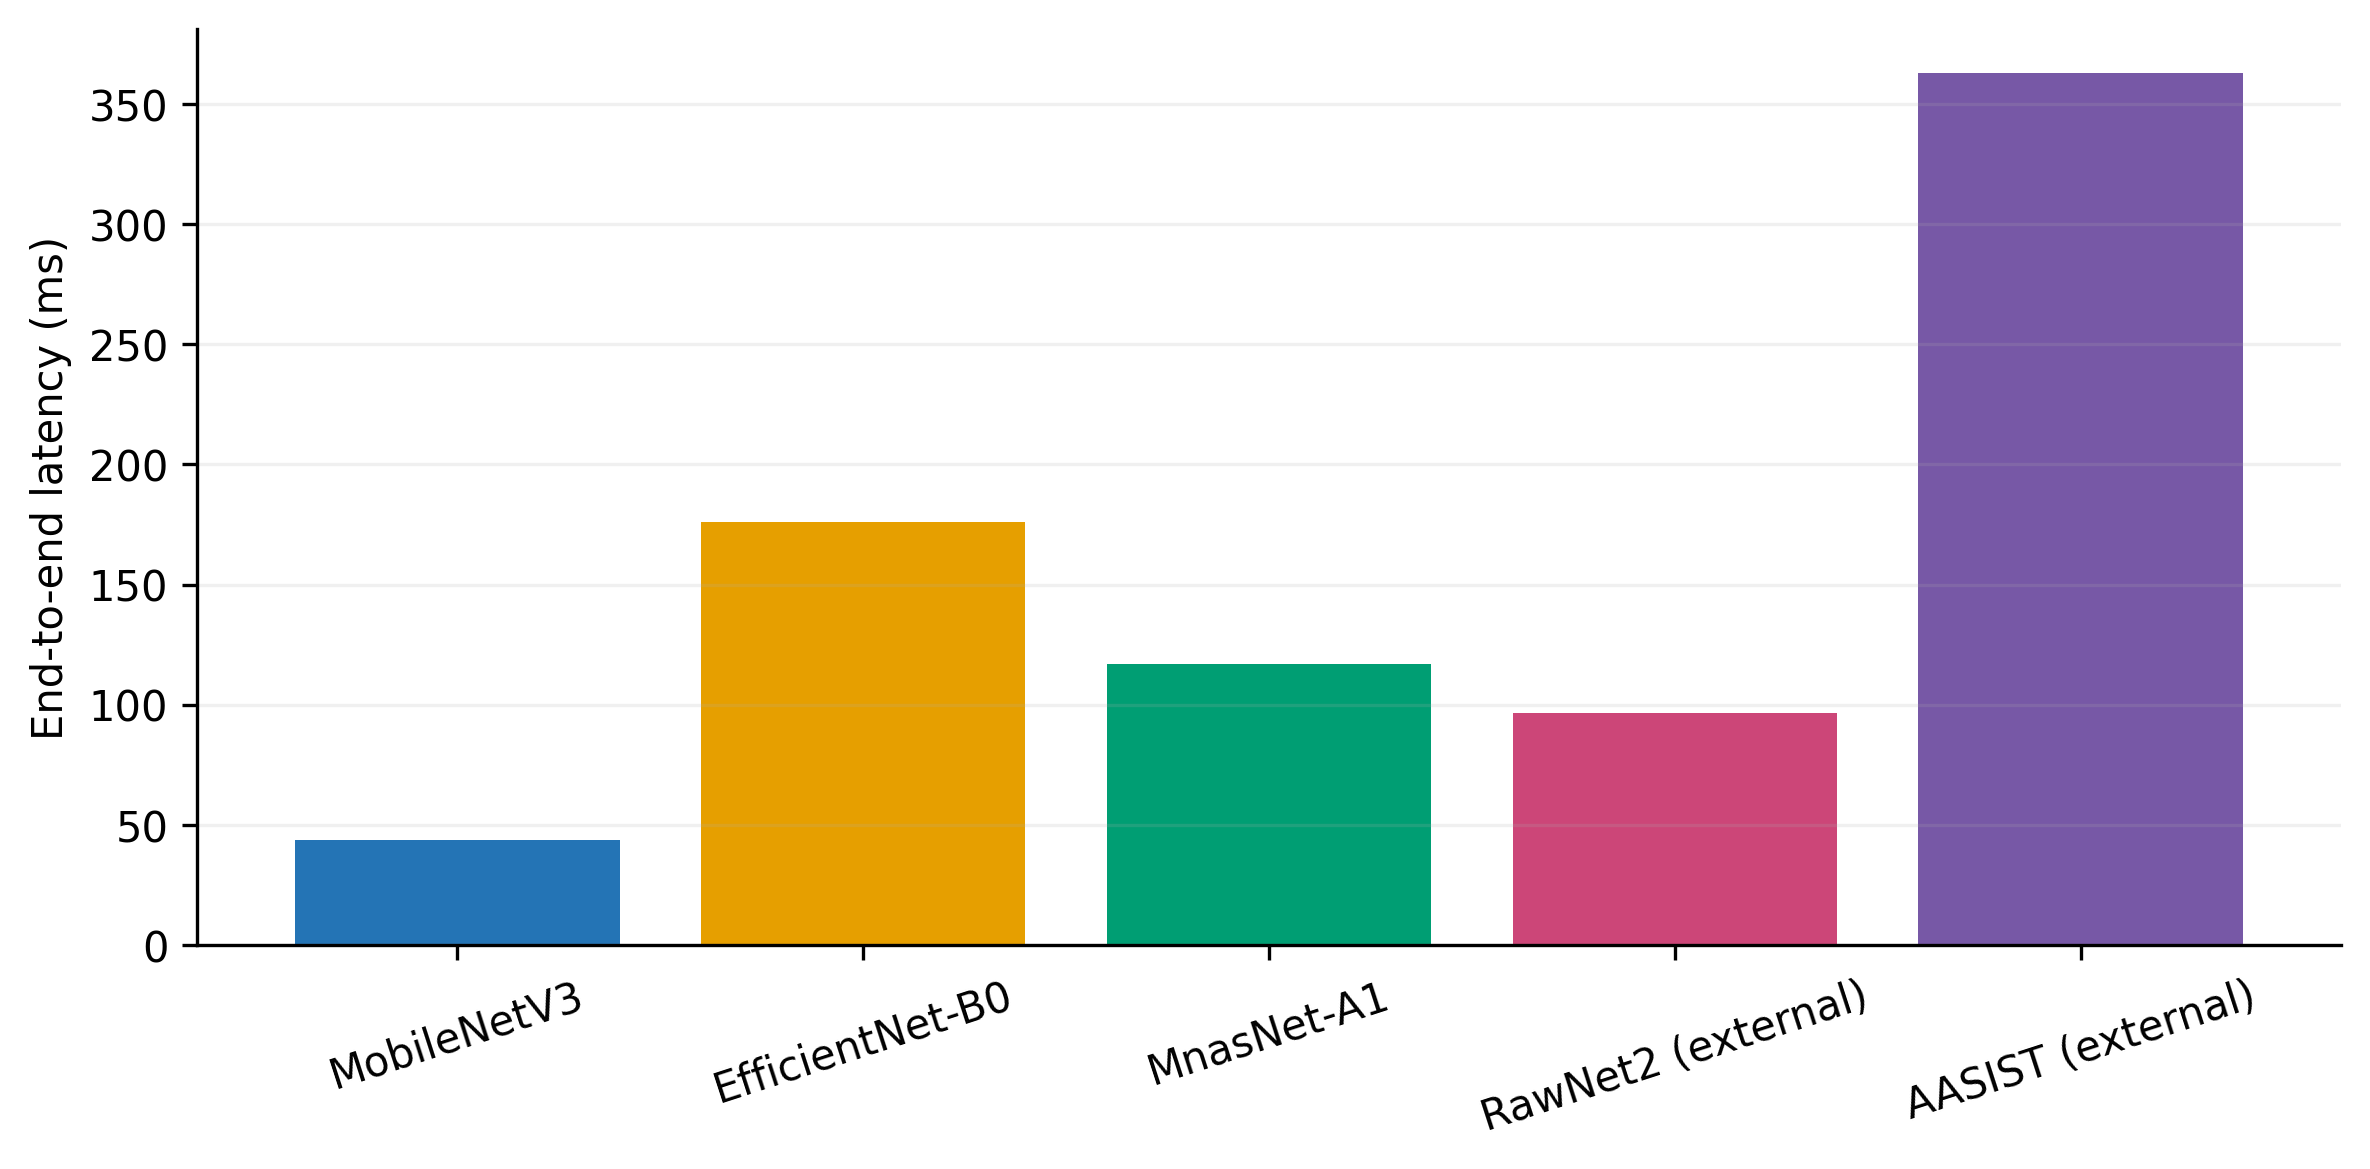
\includegraphics[width=\linewidth]{end_to_end_latency_bar.png}\caption{Measured end-to-end CPU latency.}\label{fig:lat}\end{figure}
\begin{figure}[t]\centering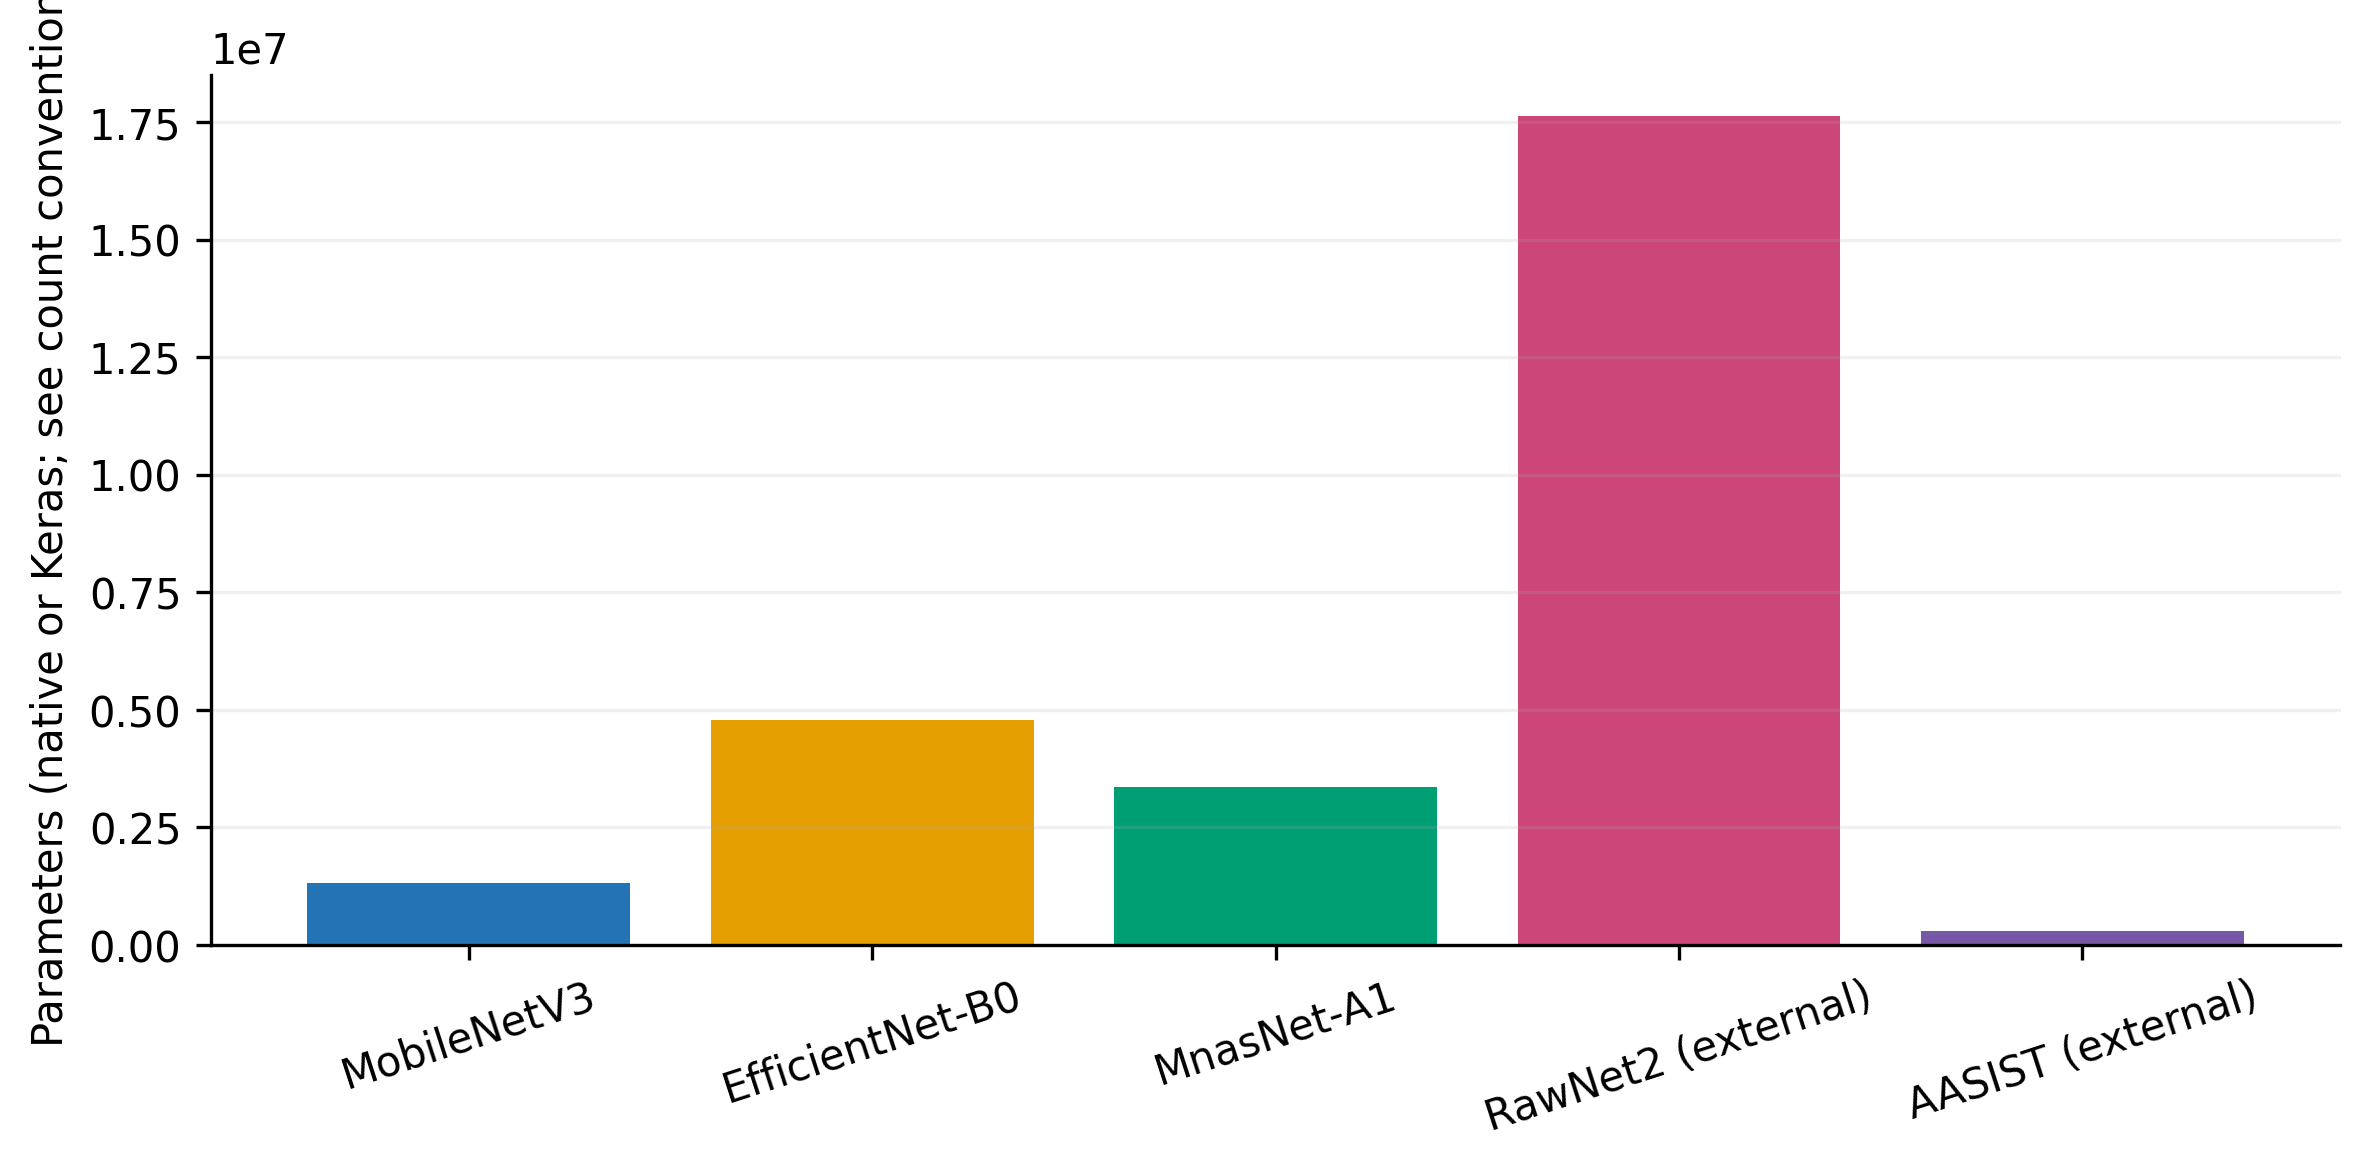
\includegraphics[width=\linewidth]{parameters_bar.png}\caption{Parameter count under the documented Keras/native conventions.}\label{fig:params}\end{figure}

\subsection{Exploratory Pareto analysis (RQ3)}
Table~\ref{tab:pareto} reports the three diagnostic objectives and the resulting frontier. MobileNet, MnasNet, RawNet2, and AASIST are diagnostic non-dominated points; EfficientNet is dominated by MobileNet. Reference membership partly reflects low clean baselines and does not constitute a quality ranking. Figure~\ref{fig:pareto} is subset-specific; official full-test Pareto is NOT\_RUN.
\begin{table}[t]\caption{Diagnostic three-objective Pareto result.}\label{tab:pareto}\centering\small
\begin{tabular}{lrrrl}\toprule Model&EER&Mean $\Delta F1$&RTF&Front\\\midrule
MobileNet&.0476&.3099&.0146&Yes\\
EfficientNet&.0476&.3650&.0586&No\\
MnasNet&.0476&.2989&.0390&Yes\\
RawNet2&.4138&.2241&.0239&Yes\\
AASIST&.3810&-.0402&.0899&Yes\\\bottomrule
\end{tabular}\end{table}
\begin{figure}[t]\centering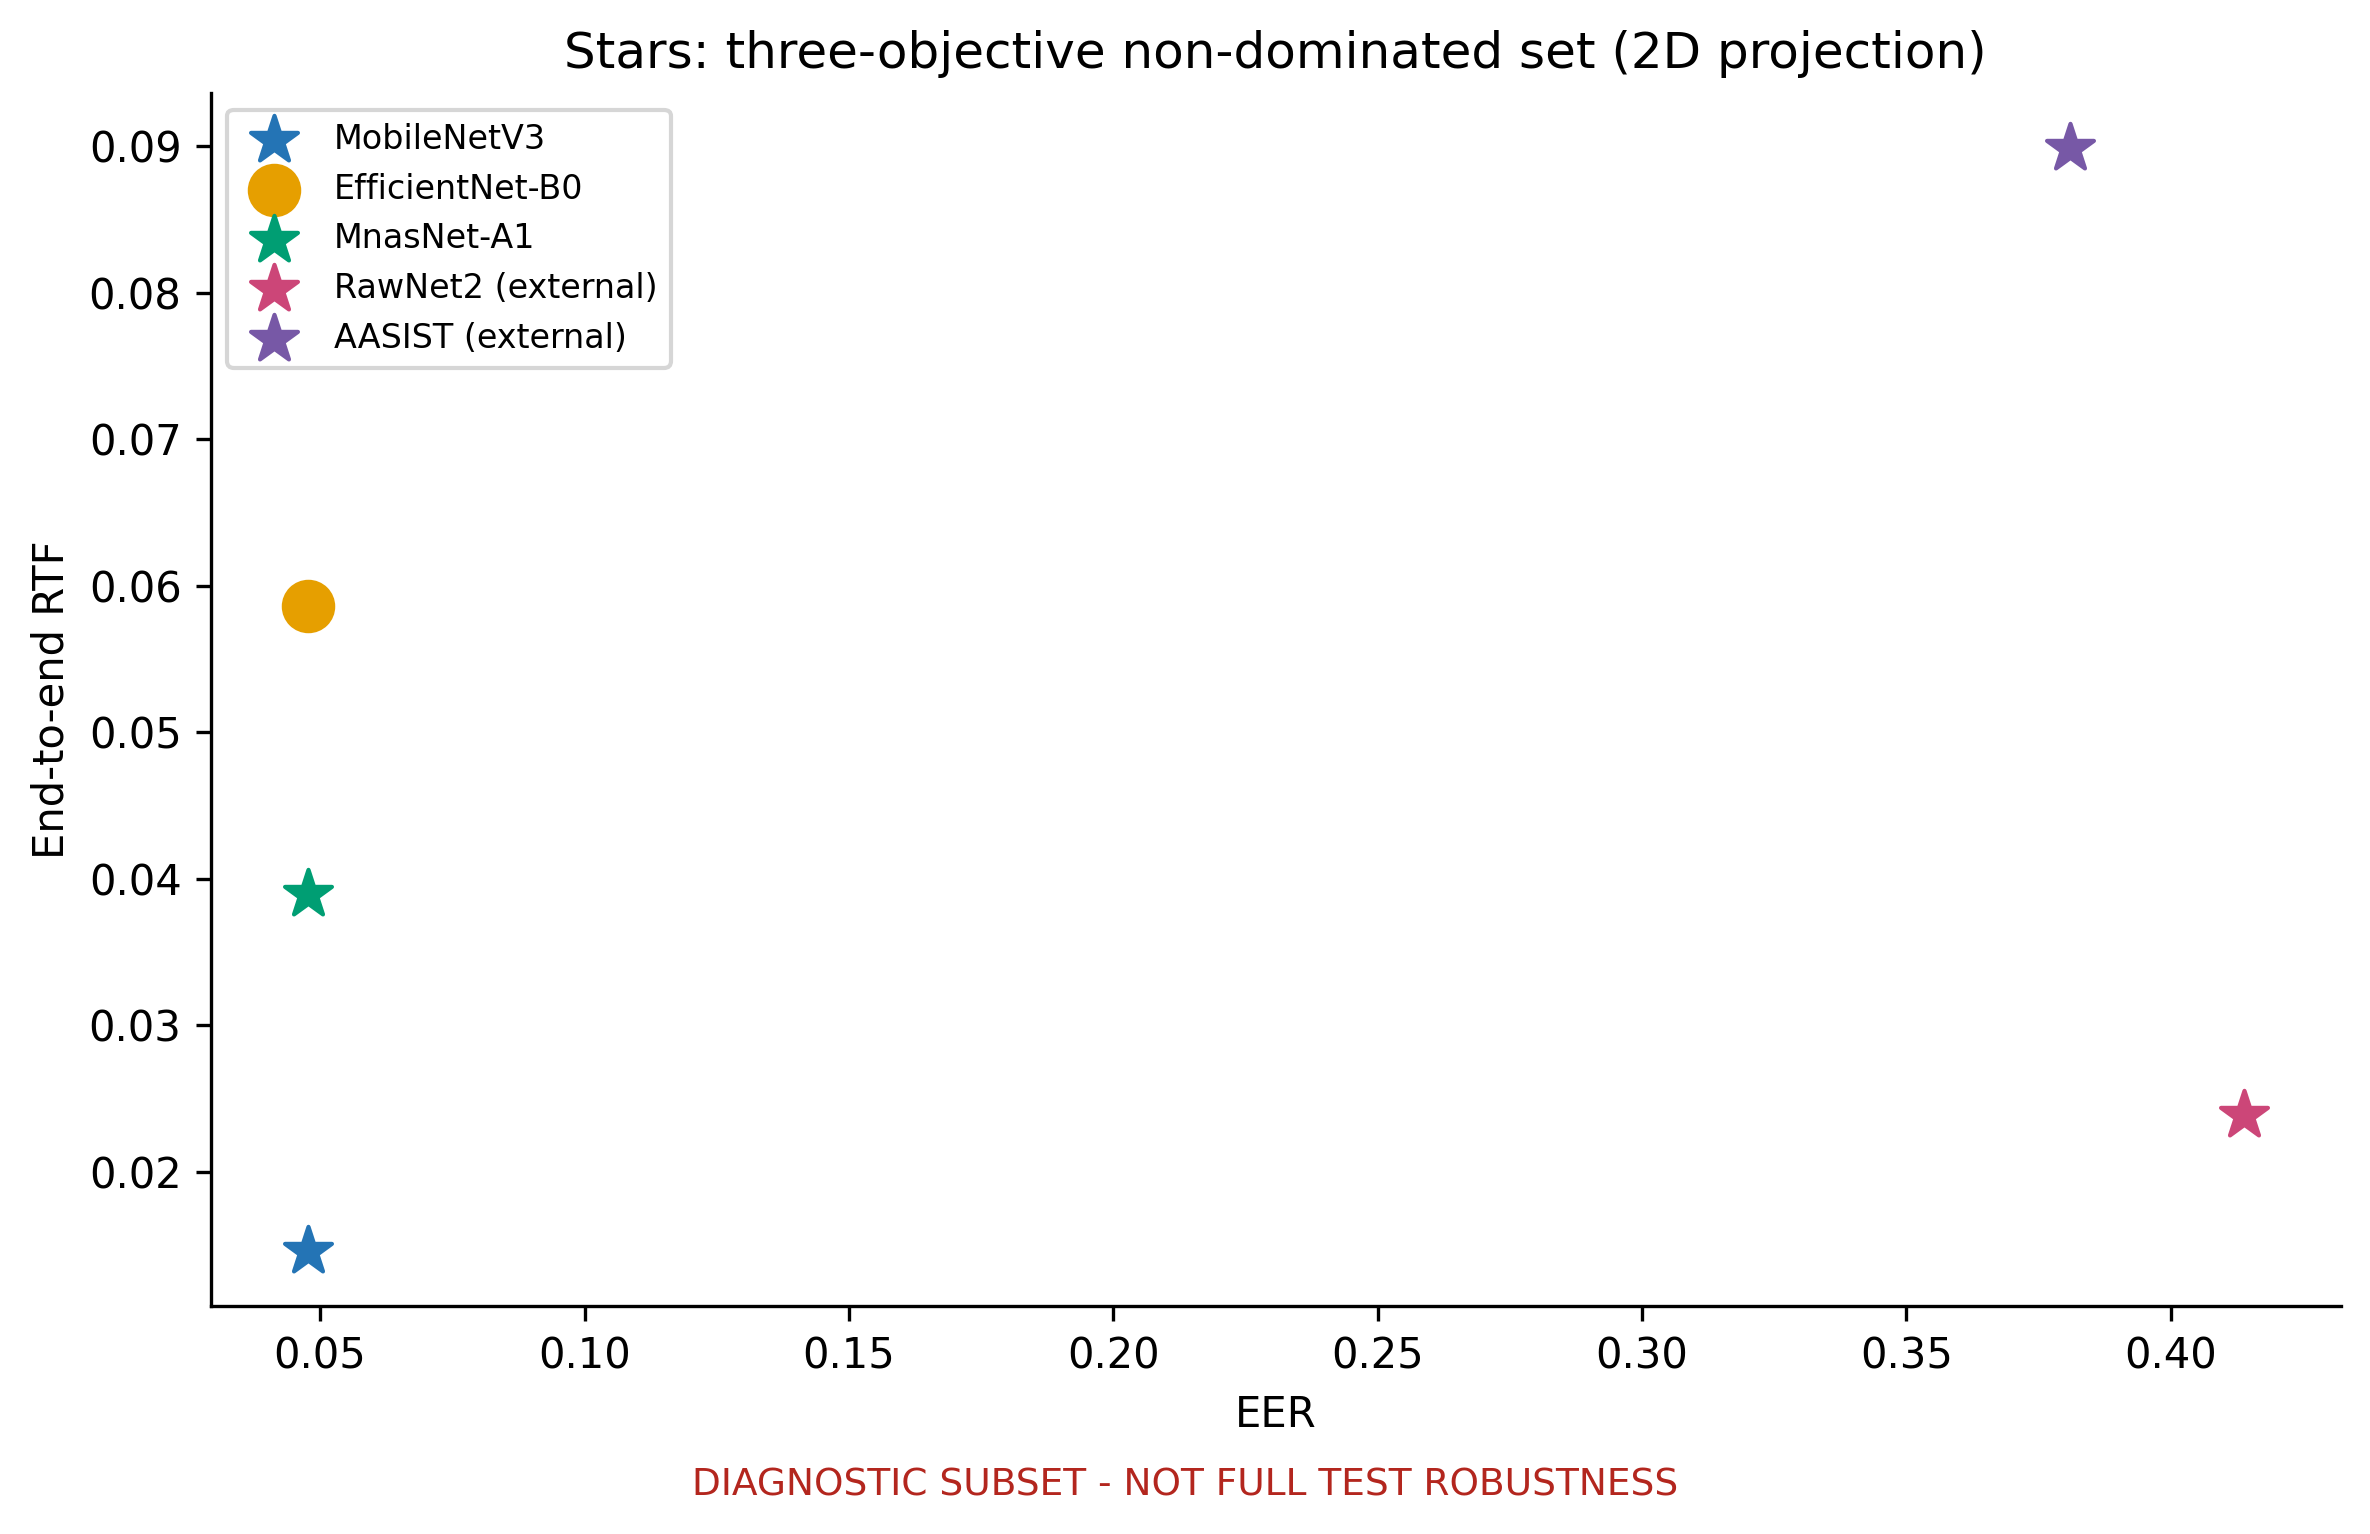
\includegraphics[width=\linewidth]{pareto_2d_eer_rtf.png}\caption{Diagnostic EER--RTF projection; stars denote the three-objective frontier.}\label{fig:pareto}\end{figure}

\subsection{Errors and uncertainty}
All models were correct on 912 samples and wrong on 11. Lightweight systems were unanimously correct while both references were wrong on 788 samples; the reverse occurred on eight. Lightweight pairwise agreement was 0.962--0.972, versus approximately 0.488--0.492 with RawNet2 and 0.555--0.558 with AASIST. Figure~\ref{fig:agree} shows the matrix.
\begin{figure}[t]\centering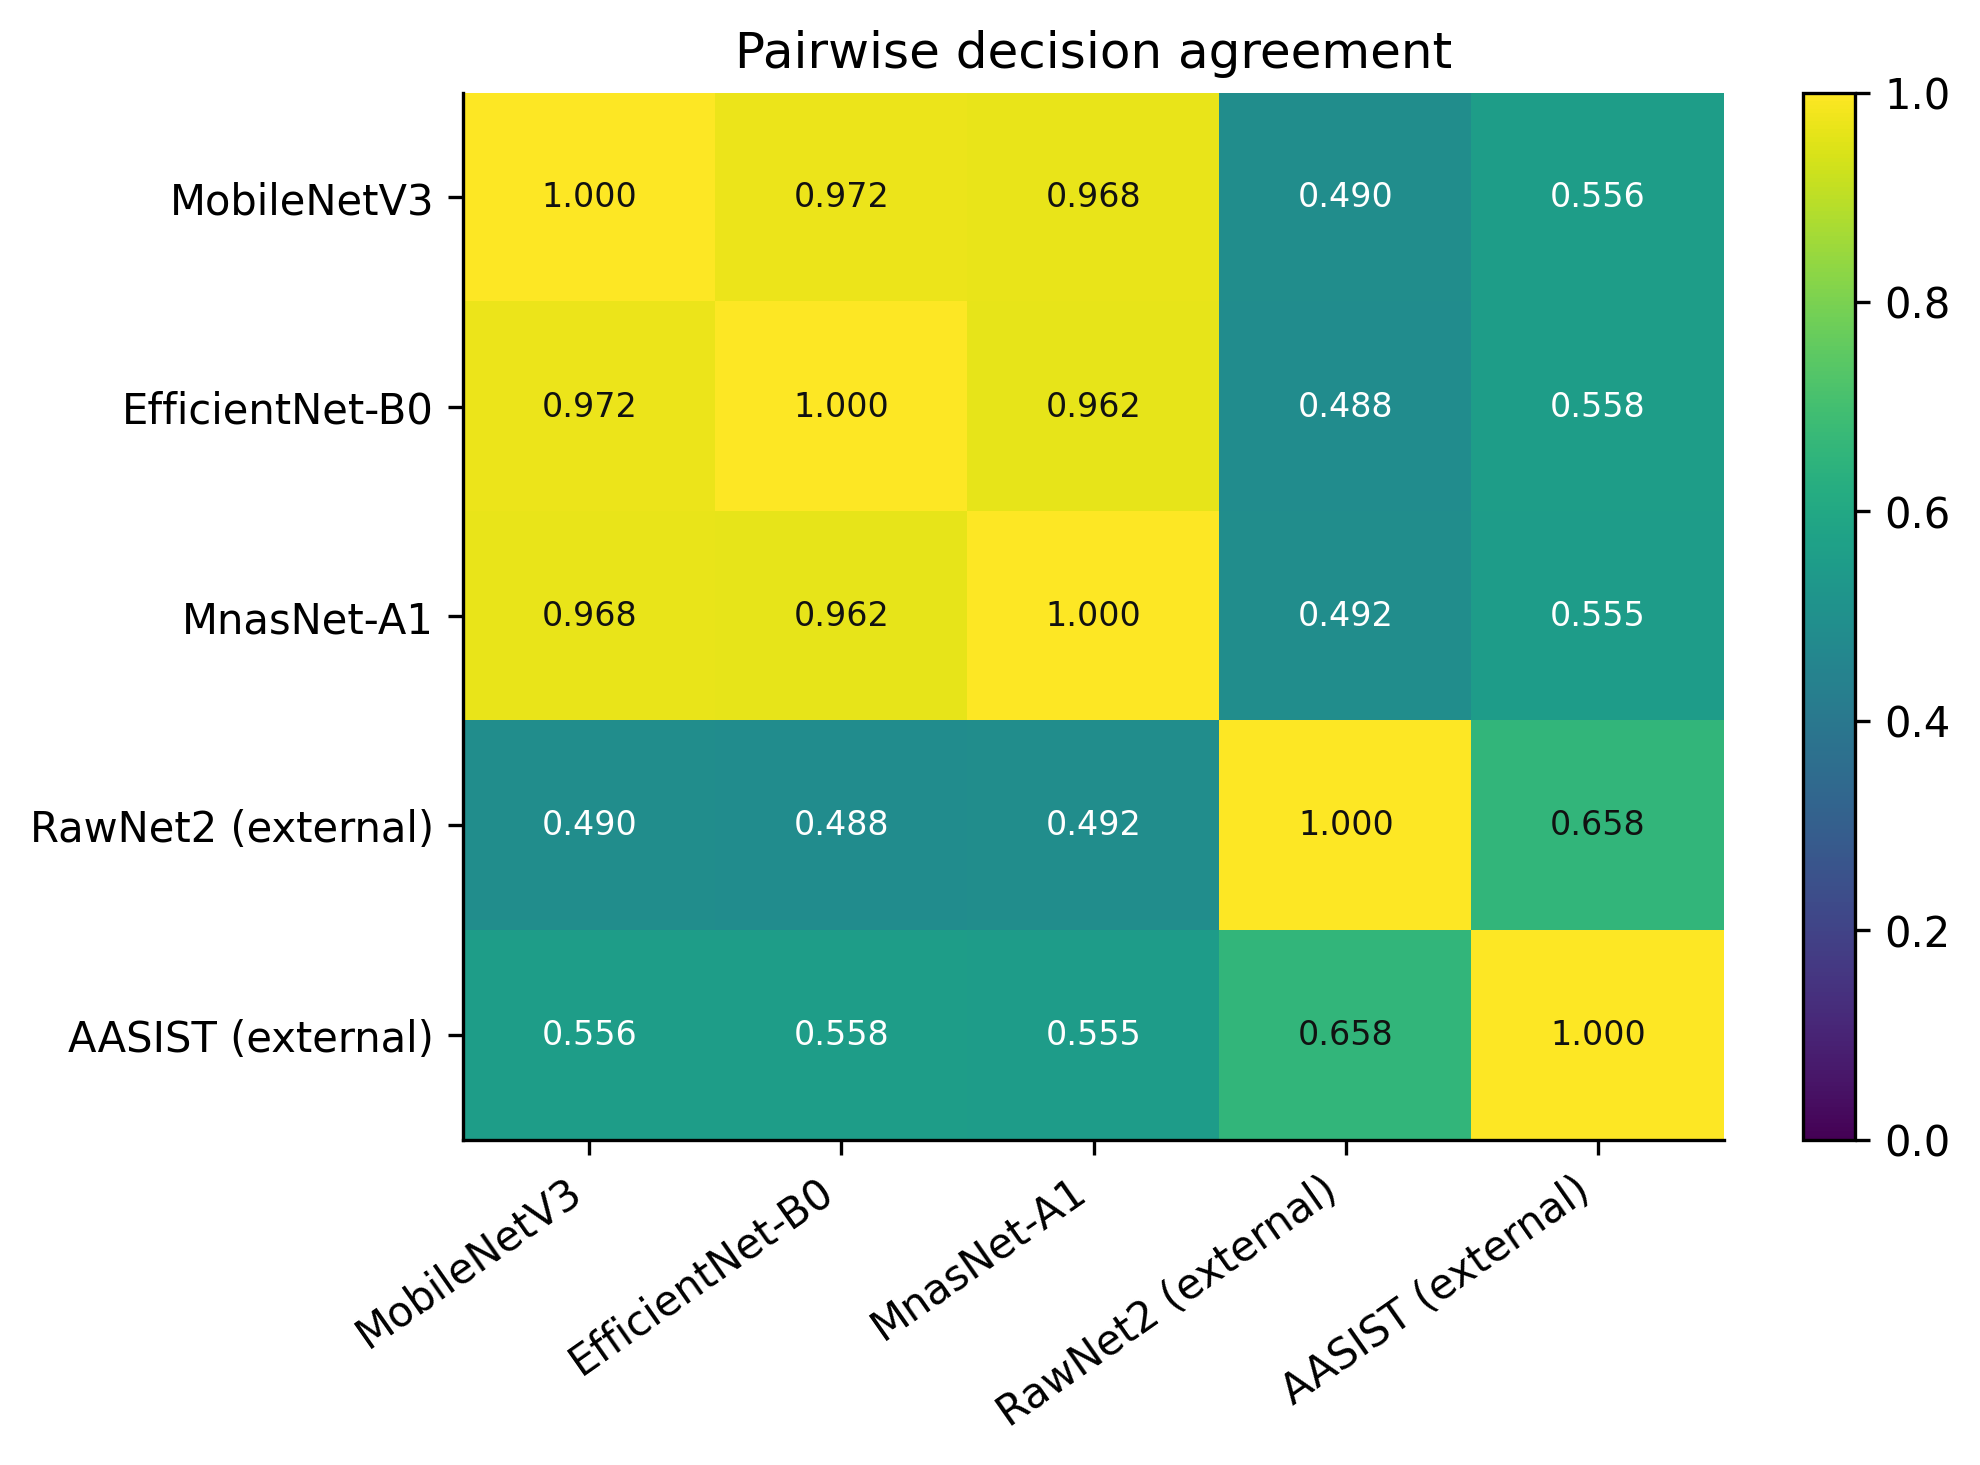
\includegraphics[width=\linewidth]{model_agreement_heatmap.png}\caption{Full-test pairwise prediction agreement.}\label{fig:agree}\end{figure}
Table~\ref{tab:ci} gives the 95\% test-set bootstrap intervals. They quantify sampling uncertainty for fixed checkpoints, not training-seed uncertainty.
\begin{table*}[t]\caption{Test-set stratified-bootstrap 95\% confidence intervals (1,000 replicates).}\label{tab:ci}\centering\small
\begin{tabular}{lccc}\toprule Model&F1 95\% CI&AUC 95\% CI&EER 95\% CI\\\midrule
MobileNet&[.9654,.9788]&[.9871,.9947]&[.0178,.0311]\\
EfficientNet&[.9477,.9651]&[.9833,.9917]&[.0311,.0482]\\
MnasNet&[.9573,.9717]&[.9842,.9923]&[.0250,.0379]\\
RawNet2&[.5150,.5489]&[.4944,.5395]&[.4616,.5016]\\
AASIST&[.4928,.5349]&[.5377,.5815]&[.4279,.4660]\\\bottomrule
\end{tabular}\end{table*}

\section{Discussion}
RQ1 shows strong clean performance for local lightweight models, with MobileNet providing the best measured quality/runtime combination. This does not contradict reference publications because domain, adapter and threshold policies differ. RQ2 shows codec resilience but substantial low-SNR sensitivity. RQ3 demonstrates that Pareto membership is not a scalar ranking: weak clean baselines can exhibit low calculated degradation. Full-test robustness and additional domains are necessary before model selection claims.

\section{Limitations}
The scope is five models and excludes pending ShuffleNet. Provenance is heterogeneous; EfficientNet is warm-up-only and RawNet2/AASIST are external. Unknown speaker/source/generator metadata limits the split to checksum-group-disjoint. Robustness uses 100 samples, synthetic white noise and simulated rather than physical replay. No unseen dataset exists. Reference preprocessing differs from original loaders and default thresholds are uncalibrated. Timing covers one Windows desktop CPU, not edge hardware; RSS is process-level. Checkpoints are single runs and bootstrap is not training-seed uncertainty. Prior development-time test inspection may weaken strict holdout interpretation.

\section{Conclusion}
LAVA provides a traceable evaluation boundary across heterogeneous anti-spoofing models. MobileNet obtained the best full-clean aggregate and CPU latency. Diagnostic stress suggests codec tolerance but white-noise fragility in lightweight detectors. The exploratory Pareto result illustrates deployment trade-offs without a weighted score. Full-test stress, physical replay, unseen data, edge devices, multiple seeds, and a valid ShuffleNet artifact are required before full six-model LAVA claims.

\section*{Acknowledgements}
Software and artifacts were developed by Phan Khac Anh Tuan, Nguyen Phuong Chinh, Lai Thanh Dat, Nguyen Tan Khiem, and Truong Thanh Dat. No external financial support is claimed.

\appendices\section{Reproducibility}
Canonical manifests are in \texttt{data/manifests}; model specifications/adapters in \texttt{src/lava}; artifacts in \texttt{models}; full clean scores/timing in \texttt{outputs/lava\_5}; and diagnostic stress/Pareto in \texttt{outputs/lava\_5/diagnostic\_100}. The benchmark runner, stress generator, report generator, and acceptance checker recompute and verify all reported values without invoking training.

\bibliographystyle{IEEEtran}\bibliography{references}
\end{document}
